
\جزوحصہء{بغیر ریمان تکمل والے تفاعل}
غیر استمراری تفاعل، ما سوائے چند، نا قابل تکمل ہیں۔ مثلاً درج ذیل تفاعل کا \عددی{[0,1]} پر کوئی ریمان تکمل نہیں پایا جاتا ہے۔
\begin{align*}
f(x)=\begin{cases}
1,&\text{\RL{ناطق}}\\
0,&\text{\RL{غیر ناطق}}
\end{cases}
\end{align*}
وقفہ \عددی{[0,1]} کے کسی بھی خانہ بندی \عددی{P} کے لئے بالائی مجموعہ اور زیریں مجموعہ درج ذیل ہوں گے۔
\begin{align*}
H&=\sum k_H\Delta x_k=\sum 1\cdot \Delta x_k=\sum \Delta x_k=1,\\
L&=\sum k_L\Delta x_k=\sum 0\cdot \Delta x_k=0
\end{align*}
وقفہ \عددی{[0,1]} پر \عددی{f} کے تکمل کی موجودگی کے لئے ضروری ہے کہ \عددی{\norm{P}\to 0}  سے \عددی{H} اور \عددی{L} کی ایک جیسی   تحدیدی قیمتیں حاصل ہوں۔ لیکن ایسا نہیں ہے:
\begin{align*}
\lim_{\norm{P}\to 0}L&=0,\quad \lim_{\norm{P}\to 0}H=1
\end{align*}
یوں \عددی{[0,1]} پر \عددی{f} کا تکمل نہیں پایا جاتا ہے۔ مستقل مضرب \عددی{kf} کا بھی تکمل نہیں پایا جاتا ہے ماسوائے جب \عددی{k} صفر ہو۔

\جزوحصہء{اصطلاحات}
علامت \عددی{\int_a^bf(x)\dif x} کے ساتھ بہت ساری اصطلاح وابستہ ہیں۔ یوں  \عددی{\int} کو \اصطلاح{علامت تکمل} کہتے ہیں، \عددی{a} تکمل کا \اصطلاح{زیریں حد} جبکہ \عددی{b} تکمل کا \اصطلاح{بالائی حد} ہے، \عددی{f} \اصطلاح{متکمل} ہے، \عددی{x} تکمل کا \اصطلاح{متغیر} ہے، جبکہ  \عددی{\int_a^bf(x)\dif x} سے مراد \عددی{a} تا \عددی{b} تفاعل \عددی{f} کا \اصطلاح{تکمل} ہے۔ تکمل حل کرنے سے مراد تکمل کی قیمت کی تلاش ہے۔
\begin{center}
\begin{tikzpicture}[font=\small]
%\draw[thick](-1,-1) grid (1,1);
%\draw[thin,gray,step=0.1](-1,-1) grid (1,1);
\draw(0,0)node[]{$\int\limits_a^b f(x)\dif x$};
\draw(-0.5,0.4)node[pin=135:{\RL{تکمل کا \موٹا{بالائی حد}}}]{};
\draw(-0.6,-0.4)node[pin=-135:{\RL{تکمل کا \موٹا{زیریں حد}}}]{};
\draw(-0.5,0)node[pin=155:{\RL{\موٹا{علامت تکمل}}}]{};
\draw(0,0.1)node[pin=70:{\RL{\موٹا{متکمل}}}]{};
\draw(0.6,0)node[pin=20:{\RL{\موٹا{تکمل کا متغیر} $x$ ہے}}]{};
\draw[decoration={brace,mirror},decorate]
  (-0.7,-0.6) -- node[below,align=right]{\RL{\عددی{a} تا \عددی{b} تفاعل}\\   \RL{\عددی{f} کا \موٹا{تکمل}}} 
(0.7,-0.6);
\end{tikzpicture}
\end{center}
کسی بھی مخصوص وقفہ پر قطعی تکمل کی قیمت تفاعل پر منحصر ہوتی ہے نا کہ غیر تابع متغیر کی علامت پر۔ یوں تکمل میں غیر تابع متغیر کو \عددی{x} کی بجائے \عددی{u} یا \عددی{t} سے ظاہر کرتے ہوئے
\begin{align*}
\text{\RL{لکھا جائے گا۔}}\quad\int_a^bf(t)\dif t\quad \text{یا}\quad \int_a^bf(u)\dif u\quad \text{\RL{کی بجائے }}\int_a^bf(x)\dif x
\end{align*} 
ان تینوں تکمل سے مراد ریمان مجموعہ ہے لہٰذا غیر تابع متغیر کا تکمل کی قیمت پر کوئی اثر نہیں ہو گا اور  تینوں تکمل  کی قیمت ایک دوسرے جیسی ہو گی۔ اسی لیے تکمل کے متغیر کو \اصطلاح{نقلی متغیر}\فرہنگ{متغیر!نقلی}\حاشیہب{dummy variable}\فرہنگ{variable!dummy} کہتے ہیں۔

\ابتدا{مثال}
درج ذیل ریمان مجموعوں کی تحدیدی قیمت کو تکمل کی صورت میں لکھیں جہاں \عددی{P} وقفہ \عددی{[-1,3]} کی خانہ بندی ہے۔
\begin{align*}
\lim_{\norm{P}\to 0}\sum_{k=1}^n (3c_k^2-2c_k+5)\Delta x_k
\end{align*}
حل:\quad
نقطہ \عددی{c_k} پر تفاعل \عددی{f(x)=3x^2-2x+5} کی قیمت تلاش کی جا رہی ہے اور  وقفہ \عددی{[-1,3]} کی خانہ بندی کی جا رہی ہے۔ یوں ہمیں \عددی{-1} تا \عددی{3} تفاعل \عددی{f} کا تکمل درکار ہے:
\begin{align*}
\lim_{\norm{P}\to 0}\sum_{k=1}^n(3c_k^2-2c_k+5)\Delta x_k=\int_{-1}^3(3x^2-2x+5)\dif x
\end{align*}
\انتہا{مثال}
%==============

\جزوحصہء{مستقل تفاعل}
ہمیں مسئلہ \حوالہ{مسئلہ_تکمل_قطعی_تکمل_کی_موجودگی} قطعی تکمل کی قیمت کے حصول کے بارے میں کچھ نہیں کہتا ہے ماسوائے چند مخصوص صورتوں میں جہاں ایک دوسرا مسئلہ زیر استعمال ہو گا۔ مستقل تفاعل ان مخصوص صورتوں میں سے ایک ہے۔ اگر ہم فرض کریں کہ وقفہ \عددی{[a,b]} پر \عددی{f} ایک مستقل تفاعل \عددی{f(x)=c} ہو تب \عددی{c_k} کی کسی بھی انتخاب کے لئے درج ذیل ہو گا۔
\begin{align*}
\sum_{k=1}^nf(c_k)\Delta x_k&=\sum_{k=1}^n c\cdot \Delta x_k&&\text{\RL{$f(c_k)$ ہر نقطہ پر $c$ کے برابر ہے}}\\
&=c\cdot \sum_{k=1}^n\Delta x_k&&\text{\RL{مجموعہ کا قاعدہ برائے مستقل مضرب}}\\
&=c(b-a)&&\text{\RL{$\sum_{k=1}^n\Delta x_k$ وقفہ $[a,b]$ کی لمبائی $b-a$ ہے}}
\end{align*}
چونکہ تمام مجموعوں کی قیمت ان کی تحدیدی قیمت \عددی{c(b-a)} کے برابر ہے  لہٰذا تکمل کی قیمت بھی یہی ہو گی۔یوں درج ذیل درست ہو گا۔

وقفہ \عددی{[a,b]} جس پر تفاعل \عددی{f(x)} کی قیمت مستقل \عددی{c} ہے کا تکمل درج ذیل ہو گا۔
\begin{align*}
\int_a^bf(x)\dif x=\int_a^bc\dif x=c(b-a)
\end{align*}

\ابتدا{مثال}
\begin{enumerate}[a.]
\item
$\int\limits_{-1}^{4}3\dif x=3(4-(-1))=(3)(5)=15$
\item
$\int\limits_{-1}^{4}(-3)\dif x=-3(4-(-1))=(-3)(5)=-15$
\end{enumerate}
\انتہا{مثال}
%============

\جزوحصہء{غیر منفی تفاعل کے ترسیم کے نیچے رقبہ}
گولا کی بلندی کا اندازہ لگانے کی خاطر مثال \حوالہ{مثال_تکمل_گولا_طے_فاصلہ_مجموعہ} میں مجموعہ کی ترکیب استعمال کی گئی جو وقفہ \عددی{[0,3]} پر  گولا کی تفاعل رفتار
\begin{align*}
v=f(t)=160-9.8t
\end{align*}
 کے ریمان مجموعے تھے۔ شکل \حوالہ{شکل_تکمل_ریمان_مجموعہ_رفتار_تفاعل} میں \عددی{t} محور اور تفاعل \عددی{v=160-9.8t} کے بیچ رقبہ کو مستطیلوں سے ظاہر کرنا دکھایا گیا ہے۔اس ذوزنقہ رقبہ کا قد \عددی{3}، زیریں قاعدہ \عددی{160} اور بالائی قاعدہ \عددی{130.6} ہے۔ جیسے جیسے خانہ بندی کا معیار صفر تک پہنچتا ہے، اتنا اصل رقبہ پر مستطیل بہتر  بیٹھتے ہیں۔ذوزنقہ کا اصل رقبہ درج ذیل ہے۔ 
\begin{align*}
\text{رقبہ}=\text{قد}\cdot\frac{\text{\RL{زیریں قاعدہ+بالائی قاعدہ}}}{2}=3\cdot\frac{130.6+160}{2}=435.9
\end{align*}
آپ کو یاد ہو گا کہ مثال \حوالہ{مثال_تکمل_گولا_طے_فاصلہ_مجموعہ} میں مجموعوں کی تحدیدی قیمت \عددی{435.6} تھی۔ہم تکمل کی قیمت بھی معلوم کر سکتے ہیں:
\begin{align*}
\int_0^3(160-9.8t)\dif t=\text{\RL{رقبہ ذوزنقہ}}=435.9
\end{align*}

\begin{figure}
\centering
\begin{tikzpicture}[font=\small,declare function={f(\x)=160-9.8*\x;},x=1.25cm,y=0.02cm]
\draw[-latex](-0.85,0)--(4,0)node[right]{$t$};
\draw[-latex](0,-0.2)--(0,180)node[above]{$v$};
\draw[domain=0:3] plot ({\x},{f(\x)});
\foreach \x in {0,1,2,3,...,14}{\pgfmathsetmacro{\y}{f(0.2*\x)};\draw(0.2*\x,\y)--++(0.2,0)--++(0,-\y);}
\foreach \x in {1,2,3}{\draw(\x,0)node[below]{$\x$}--++(0,0.2);}
\foreach \y in {40,80,120,160}{\draw(0,\y)node[left]{\y}--++(0.2,0);}
\draw(1,160)node[right]{$v=160-9.8t$};
\draw(0,-25)--++(0,-10) (3,-25)--++(0,-10);
\draw[stealth-stealth](0,-30)--++(3,0)node[pos=0.5,fill=white]{\text{قد}};
\draw[stealth-stealth](-0.75,0)--++(0,160)node[pos=0.5,fill=white]{قاعدہ};
\draw[stealth-stealth](3.5,0)--++(0,130.6)node[pos=0.5,fill=white]{قاعدہ};
\draw(-0.75+0.1,160)--++(-0.2,0) (3.5-0.1,130.6)--++(0.2,0);
\end{tikzpicture}
\caption{وقفہ $[0,3]$ پر سمتی رفتار تفاعل $v=160-9.8t$ کے ریمان رقبہ کے لئے مستطیل۔}
\label{شکل_تکمل_ریمان_مجموعہ_رفتار_تفاعل}
\end{figure} 

ہم تکمل اور رقبہ کے تعلق کو دو طرح استعمال کر سکتے ہیں۔جب ہمیں \عددی{x} محور اور استمراری غیر منفی تفاعل \عددی{y=f(x)} کے بیچ رقبہ کا کلیہ معلوم ہو تب ہم تکمل کی قیمت اس رقبہ سے حاصل کر سکتے ہیں۔ جب ہمیں رقبہ معلوم نہ ہو تب ہم تفاعل کے تکمل سے رقبہ تلاش کر سکتے ہیں۔

\ابتدا{تعریف}
فرض کریں وقفہ \عددی{[a,b]} پر \عددی{f(x)\ge 0} استمراری ہے۔ تفاعل \عددی{f} کے ترسیم اور \عددی{x} محور کے بیچ رقبہ درج ذیل ہو گا۔
\begin{align*}
S=\int\limits_a^b f(x)\dif x
\end{align*}
\انتہا{تعریف}
%=======================

ہم نے درج بالا تعریف غیر معیاری اشکال کے لئے پیش کیا۔ کیا یہ تعریف معیاری اشکال کے لئے بھی کارآمد ہو گا؟ اس کا جواب ہے، "جی ہاں"، البتہ یہ ثابت کرنا اتنا آسان نہیں ہے اور اس پر مزید بات نہیں کی جائے گی۔

\ابتدا{مثال}\شناخت{مثال_تکمل_رقبہ_سے_تکمل_قیمت}\ترچھا{رقبہ استعمال کرتے ہوئے تکمل کی قیمت کا تلاش}\\
درج ذیل تکمل کی قیمت تلاش کریں۔
\begin{align*}
\int_a^bx\dif x, \quad 0<a<b
\end{align*}
حل:\quad
ہم خطہ \عددی{a<x<b} کے لئے \عددی{y=x} ترسیم کرتے ہیں جس سے  ذوزنقہ حاصل ہوتا ہے (شکل \حوالہ{شکل_مثال_تکمل_رقبہ_سے_تکمل_قیمت})۔ تکمل کی قیمت ذوزنقہ کی قیمت سے تلاش کرتے ہیں۔
\begin{align*}
\int_a^b x\dif x=(b-a)\cdot \frac{a+b}{2}=\frac{b^2}{2}-\frac{a^2}{2}
\end{align*}  
یوں \عددی{a=1} اور \عددی{b=\sqrt{5}} کی صورت میں درج ذیل ہو گا۔
\begin{align*}
\int_1^{\sqrt{5}} x\dif x=\frac{(\sqrt{5})^2}{2}-\frac{1^2}{2}=2
\end{align*} 
دھیان رہے کہ \عددی{x} کا الٹ تفرق \عددی{\tfrac{x^2}{2}} ہے جو تکمل اور رقبہ کے تعلق کی طرف اشارہ ہے۔ 
\انتہا{مثال}
%====================== 
\begin{figure}
\centering
\begin{minipage}{0.45\textwidth}
\centering
\begin{tikzpicture}[declare function={f(\x)=\x;}]
\pgfmathsetmacro{\ya}{f(0.25)}
\pgfmathsetmacro{\yb}{f(0.75)}
\begin{axis}[clip=false,axis on top,small,axis lines=middle,xlabel={$x$},ylabel={$y$},xlabel style={at={(current axis.right of origin)},anchor=west},ylabel style={at={(current axis.above origin)},anchor=south},xtick={0.25,0.75},xticklabels={$a$,$b$},ytick={\ya,\yb},yticklabels={$a$,$b$}]
\fill[lgray](0.25,0)--(0.25,0.25)--(0.75,0.75)--(0.75,0)--(0.25,0);
\addplot[domain=0:0.8]{f(x)}node[pos=0.5,above left]{$y=x$};
\draw(axis cs:0.25,0)--(0.25,\ya)node[pos=0.5,left]{$a$};
\draw(axis cs:0.75,0)--(0.75,\yb)node[pos=0.5,right]{$b$};
\draw[stealth-stealth](axis cs:0.25,-0.2)--(0.75,-0.2)node[pos=0.5,fill=white]{$b-a$};
\draw(axis cs:0.25,-0.15)--(axis cs:0.25,-0.25);
\draw(axis cs:0.75,-0.15)--(axis cs:0.75,-0.25);
\end{axis}
\end{tikzpicture}
\caption{خطہ برائے مثال \حوالہ{مثال_تکمل_رقبہ_سے_تکمل_قیمت}}
\label{شکل_مثال_تکمل_رقبہ_سے_تکمل_قیمت}
\end{minipage}\hfill
\begin{minipage}{0.45\textwidth}
\centering
\begin{tikzpicture}[declare function={f(\x)=\x*\x;}]
\begin{axis}[clip=false,axis on top,small,axis lines=middle,xlabel={$x$},ylabel={$y$},xlabel style={at={(current axis.right of origin)},anchor=west},ylabel style={at={(current axis.above origin)},anchor=south},xtick={0,1,2,3,4,5}, xticklabels={$x_0$,$x_1$,$x_2$,$x_3$,$x_{n-1}$,$x_n=b$},ytick={\empty},xmax=6]
\draw(axis cs:0,0)node[below,font=\footnotesize]{$x_0=a$};
\draw[fill=lgray](axis cs:0,0)rectangle(1,1);
\draw[fill=lgray](axis cs:1,0)rectangle(2,4);
\draw[fill=lgray](axis cs:2,0)rectangle(3,9);
\draw[fill=lgray](axis cs:4,0)rectangle(5,25);
\addplot[domain=0:5]{f(x)}node[pos=0.5,above left]{$y=x^2$};
\draw[stealth-stealth](axis cs:0,-4)--(axis cs:1,-4)node[pos=0.5,below]{$\Delta x$};
\draw[stealth-stealth](axis cs:1,-4)--(axis cs:2,-4)node[pos=0.5,below]{$\Delta x$};
\draw[stealth-stealth](axis cs:2,-4)--(axis cs:3,-4)node[pos=0.5,below]{$\Delta x$};
\draw[stealth-stealth](axis cs:4,-4)--(axis cs:5,-4)node[pos=0.5,below]{$\Delta x$};
\draw(axis cs:0,-3)--(axis cs:0,-5);
\draw(axis cs:1,-3)--(axis cs:1,-5);
\draw(axis cs:2,-3)--(axis cs:2,-5);
\draw(axis cs:3,-3)--(axis cs:3,-5);
\draw(axis cs:4,-3)--(axis cs:4,-5);
\draw(axis cs:5,-3)--(axis cs:5,-5);
\end{axis}
\end{tikzpicture}
\caption{ریمان مجموعوں کے مستطیل (مثال \حوالہ{مثال_تکمل_قطع_مکافی_رقبہ})}
\label{شکل_مثال_تکمل_قطع_مکافی_رقبہ}
\end{minipage}
\end{figure}

\ابتدا{مثال}\شناخت{مثال_تکمل_قطع_مکافی_رقبہ}\ترچھا{قطعی تکمل سے رقبے کا حصول}\\
قطع مکافی \عددی{y=x^2} اور \عددی{x} محور کے بیچ وقفہ \عددی{[0,b]} پر رقبہ تلاش کریں (شکل \حوالہ{شکل_مثال_تکمل_قطع_مکافی_رقبہ})۔

حل:\quad
ہم تکمل کی قیمت ریمان رقبوں کی حد سے حاصل کرتے ہیں۔ ہم (غیر معیاری) تفاعل کو ترسیم کر کے وقفہ \عددی{[0,b]} کو \عددی{n} یکساں ذیلی وقفوں میں تقسیم کرتے ہیں۔یوں ہر ذیلی وقفہ کی لمبائی \عددی{\Delta x=\tfrac{b-0}{n}=\tfrac{b}{n}} ہو گی۔ خانہ بندی کے نقطے درج ذیل ہوں گے۔
\begin{align*}
x_0=0,\quad x_1=\Delta x,\quad x_2=2\Delta x,\quad \cdots, \quad x_{n-1}=(n-1)\Delta x,\quad x_n=n\Delta x=b
\end{align*}
ہم جس طرح چاہیں \عددی{c_k} نقطے منتخب کر سکتے ہیں۔ ہم ہر ذیلی وقفہ کے دائیں سر نقطہ کو \عددی{c_k} منتخب کرتے ہیں۔یوں \عددی{c_1=x_1}، \عددی{c_2=x_2}، وغیرہ ہو گا۔ منتخب کردہ نقطوں سے حاصل مستطیلوں کے رقبے درج ذیل ہیں۔
\begin{align*}
f(c_1)\Delta x&=f(\Delta x)\Delta x=(\Delta x)^2\Delta x=(1^2)(\Delta x)^3\\
f(c_2)\Delta x&=f(2\Delta x)\Delta x=(2\Delta x)^2\Delta x=(2^2)(\Delta x)^3\\
\vdots\\
f(c_n)\Delta x&=f(n\Delta x)\Delta x=(n\Delta x)^2\Delta x=(n^2)(\Delta x)^3
\end{align*}
ان رقبوں کا مجموعہ درج ذیل ہے۔
\begin{align*}
S_n&=\sum_{k=1}^n f(c_k)\Delta x\\
&=\sum_{k=1}^n k^2(\Delta x)^3\\
&=(\Delta x)^3\sum_{k=1}^nk^2&&\text{\RL{$(\Delta x)^3$ مستقل ہے}}\\
&=\frac{b^3}{n^3}\cdot \frac{n(n+1)(2n+1)}{6}&&\text{\RL{مساوات \حوالہ{مساوات_تکمل_قاعدہ_عدد_صحیح_مجموعہ} میں $\Delta x=\tfrac{b}{n}$}}\\
&=\frac{b^3}{6}\cdot \frac{(n+1)(2n+1)}{n^2}\\
&=\frac{b^3}{6}\cdot\frac{2n^2+3n+1}{n^2}\\
&=\frac{b^3}{6}\cdot\big(2+\frac{3}{n}+\frac{1}{n^2}\big)
\end{align*}
 اب قطعی تکمل کی تعریف 
\begin{align*}
\int_a^bf(x)\dif x=\lim_{\norm{P}\to 0}\sum_{k=1}^nf(c_k)\Delta x
\end{align*}
استعمال کرتے ہوئے \عددی{x=0} تا \عددی{x=b} قطع مکافی کے نیچے رقبہ تلاش کرتے ہیں۔
\begin{align*}
\int_0^bx^2\dif x&=\lim_{n\to \infty}S_n&&\text{\RL{یہاں $\norm{P}\to 0$ سے مراد $n\to\infty$ ہے}}\\
&=\lim_{n\to\infty}\frac{b^3}{6}\cdot\big(2+\frac{3}{n}+\frac{1}{n^2}\big)&&\text{\RL{مذکورہ بالا مساوات}}\\
&=\frac{b^3}{6}\cdot(2+0+0)=\frac{b^3}{3}
\end{align*}
یوں \عددی{b=1} اور \عددی{b=1.5} کی صورت میں درج ذیل جوابات حاصل ہوں گے۔
\begin{align*}
\int_0^1x^2\dif x=\frac{1^3}{3}=\frac{1}{3},\quad \int_0^{1.5}x^2\dif x=\frac{(1.5)^3}{3}=\frac{3.375}{3}=1.125
\end{align*}
یہاں بھی دھیان رہے کہ \عددی{x^2} کا الٹ تفرق \عددی{\tfrac{x^3}{3}} ہے۔
\انتہا{مثال}
%==========================

\حصہء{سوالات}
\موٹا{سگما روپ}\\
سوال \حوالہ{سوال_تکمل_سگما_روپ_الف} تا سوال \حوالہ{سوال_تکمل_سگما_روپ_ب} میں مجموعہ کو سگما روپ میں لکھنے کے بعد اس کی قیمت تلاش کریں۔

\ابتدا{سوال}\شناخت{سوال_تکمل_سگما_روپ_الف}
$\sum\limits_{k=1}^2\tfrac{6k}{k+1}$
\انتہا{سوال}
%======================
\ابتدا{سوال}
$\sum\limits_{k=1}^3\tfrac{k-1}{k}$
\انتہا{سوال}
%=====================
\ابتدا{سوال}
$\sum\limits_{k=1}^4\cos k\pi$
\انتہا{سوال}
%=====================
\ابتدا{سوال}
$\sum\limits_{k=1}^5\sin k\pi$
\انتہا{سوال}
%=====================
\ابتدا{سوال}
$\sum\limits_{k=1}^3(-1)^{k+1}\sin\tfrac{\pi}{k}$
\انتہا{سوال}
%=====================
\ابتدا{سوال}\شناخت{سوال_تکمل_سگما_روپ_ب}
$\sum\limits_{k=1}^4 (-1)^k\cos k\pi$
\انتہا{سوال}
%=====================
\ابتدا{سوال}
درج ذیل میں سے کونسی \عددی{1+2+4+8+16+32} کی سگما علامتی روپ ہے۔
\begin{multicols}{3}
\begin{enumerate}[a.]
\item
$\sum\limits_{k=1}^62^{k-1}$
\item
$\sum\limits_{k=0}^5 2^k$
\item
$\sum\limits_{k=-1}^4 2^{k+1}$
\end{enumerate}
\end{multicols}
\انتہا{سوال}
%=========================
\ابتدا{سوال}
درج ذیل میں سے کونسی \عددی{1-2+4-8+16-32} کی سگما علامتی روپ ہے۔
\begin{multicols}{3}
\begin{enumerate}[a.]
\item
$\sum\limits_{k=1}^6(-2)^{k-1}$\\
\item
$\sum\limits_{k=0}^5 (-1)^k2^k$
\item
$\sum\limits_{k=-2}^3 (-1)^{k+1}2^{k+2}$
\end{enumerate}
\end{multicols}
\انتہا{سوال}
%=========================
\ابتدا{سوال}
درج ذیل میں سے کونسا کلیہ باقی دو کلیات سے مختلف ہے؟
\begin{multicols}{3}
\begin{enumerate}[a.]
\item
$\sum\limits_{k=2}^4 \tfrac{(-1)^{k-1}}{k-1}$
\item
$\sum\limits_{k=0}^2 \tfrac{(-1)^k}{k+1}$
\item
$\sum\limits_{k=-1}^1 \tfrac{(-1)^k}{k+2}$
\end{enumerate}
\end{multicols}
\انتہا{سوال}
%=======================
\ابتدا{سوال}
درج ذیل میں سے کونسا کلیہ باقی دو کلیات سے مختلف ہے؟
\begin{multicols}{3}
\begin{enumerate}[a.]
\item
$\sum\limits_{k=1}^4 (k-1)^2$
\item
$\sum\limits_{k=-1}^3 (k+1)^2$
\item
$\sum\limits_{k=-3}^{-1} k^2$
\end{enumerate}
\end{multicols}
\انتہا{سوال}
%=======================
سوال \حوالہ{سوال_تکمل_سگما_روپ_لکھائی_الف} تا سوال \حوالہ{سوال_تکمل_سگما_روپ_لکھائی_ب} میں دیے مجموعوں کو سگما روپ میں لکھیں۔ آپ کے جواب کی صورت مجموعی سلسلہ کی زیریں حد پر منحصر ہو گا۔ 

\ابتدا{سوال}\شناخت{سوال_تکمل_سگما_روپ_لکھائی_الف}
$1+2+3+4+5+6$
\انتہا{سوال}
%======================
\ابتدا{سوال}
$1+4+9+16$
\انتہا{سوال}
%======================
\ابتدا{سوال}
$\tfrac{1}{2}+\tfrac{1}{4}+\tfrac{1}{8}+\tfrac{1}{16}$
\انتہا{سوال}
%======================
\ابتدا{سوال}
$2+4+6+8+10$
\انتہا{سوال}
%======================
\ابتدا{سوال}
$1-\tfrac{1}{2}+\tfrac{1}{3}-\tfrac{1}{4}+\tfrac{1}{5}$
\انتہا{سوال}
%======================
\ابتدا{سوال}\شناخت{سوال_تکمل_سگما_روپ_لکھائی_ب}
$-\tfrac{1}{5}+\tfrac{2}{5}-\tfrac{3}{5}+\tfrac{4}{5}-\tfrac{5}{5}$
\انتہا{سوال}
%======================
\موٹا{متناہی مجموعہ کی قیمت}\\
\ابتدا{سوال}
فرض کریں کہ \عددی{\sum\limits_{k=1}^n a_k=-5} اور \عددی{\sum\limits_{k=1}^nb_k=6} ہیں۔ درج ذیل کی قیمتیں تلاش کریں۔
\begin{multicols}{3}
\begin{enumerate}[a.]
\item
$\sum\limits_{k=1}^n 3a_k$
\item
$\sum\limits_{k=1}^n\tfrac{b_k}{6}$
\item
$\sum\limits_{k=1}^n (a_k+b_k)$
\item
$\sum\limits_{k=1}^n(a_k-b_k)$
\item
$\sum\limits_{k=1}^n(b_k-2a_k)$
\end{enumerate}
\end{multicols}
\انتہا{سوال}
%=======================
\ابتدا{سوال}
فرض کریں کہ \عددی{\sum\limits_{k=1}^n a_k=0} اور \عددی{\sum\limits_{k=1}^n b_k=1} ہیں۔ درج ذیل کی قیمتیں تلاش کریں۔
\begin{multicols}{4}
\begin{enumerate}[a.]
\item
$\sum\limits_{k=1}^n 8a_k$
\item
$\sum\limits_{k=1}^n250b_k$
\item
$\sum\limits_{k=1}^n(a_k+1)$
\item
$\sum\limits_{k=1}^n(b_k-1)$
\end{enumerate}
\end{multicols}
\انتہا{سوال}
%========================
سوال \حوالہ{سوال_تکمل_قواعد_مجموعی_الجبرا_الف} تا سوال \حوالہ{سوال_تکمل_قواعد_مجموعی_الجبرا_ب} میں دیے گئے الجبرائی فقروں کی قیمتوں کو صفحہ \حوالہصفحہ{جزوحصہ_تکمل_متناہی_مجموعہ_کی_الجبرا} پر دیے گئے متناہی مجموعہ کے  الجبرائی قواعد اور مساوات \حوالہ{مساوات_تکمل_قاعدہ_عدد_صحیح_مجموعہ} میں دیے کلیات کی مدد سے تلاش کریں۔
 
\ابتدا{سوال}\شناخت{سوال_تکمل_قواعد_مجموعی_الجبرا_الف}
\begin{multicols}{3}
\begin{enumerate}[a.]
\item
$\sum\limits_{k=1}^{10} k$
\item
$\sum\limits_{k=1}^{10}k^2$
\item
$\sum\limits_{k=1}^{10}k^3$
\end{enumerate}
\end{multicols}
\انتہا{سوال}
%=====================
\ابتدا{سوال}
\begin{multicols}{3}
\begin{enumerate}[a.]
\item
$\sum\limits_{k=1}^{13} k$
\item
$\sum\limits_{k=1}^{13}k^2$
\item
$\sum\limits_{k=1}^{13}k^3$
\end{enumerate}
\end{multicols}
\انتہا{سوال}
%=====================
\ابتدا{سوال}
$\sum\limits_{k=1}^7 (-2k)$
\انتہا{سوال}
%==================
\ابتدا{سوال}
$\sum\limits_{k=1}^5 \tfrac{\pi k}{15}$
\انتہا{سوال}
%==================
\ابتدا{سوال}
$\sum\limits_{k=1}^6 (3-k^2)$
\انتہا{سوال}
%==================
\ابتدا{سوال}
$\sum\limits_{k=1}^6 (k^2-5)$
\انتہا{سوال}
%==================
\ابتدا{سوال}
$\sum\limits_{k=1}^5 k(3k+5)$
\انتہا{سوال}
%==================
\ابتدا{سوال}
$\sum\limits_{k=1}^7 k(2k+1)$
\انتہا{سوال}
%==================
\ابتدا{سوال}
$\sum\limits_{k=1}^5 \tfrac{k^3}{225}+\big(\sum\limits_{k=1}^5 k\big)^3$
\انتہا{سوال}
%==================
\ابتدا{سوال}\شناخت{سوال_تکمل_قواعد_مجموعی_الجبرا_ب}
$\big(\sum\limits_{k=1}^7 k\big)^2-\sum\limits_{k=1}^7 \tfrac{k^3}{4}$
\انتہا{سوال}
%==================
\موٹا{ریمان مجموعوں کے لئے مستطیلیں}\\
سوال \حوالہ{سوال_تکمل_ریمان_مستطیل_شمول_الف} تا سوال \حوالہ{سوال_تکمل_ریمان_مستطیل_شمول_ب} میں تفاعل \عددی{f(x)} کو دیے گئے وقفے پر ترسیم کریں۔ وقفے کی ایک جتنے لمبے چار ذیلی وقفوں میں خانہ بندی کریں۔ترسیم پر ریمان مجموعہ \عددی{\sum_{k=1}^4f(c_k)\Delta x_k} کے ساتھ وابستہ مستطیل دکھائیں جہاں \عددی{k} ویں  ذیلی وقفہ کا  (ا) بایاں سر نقطہ، (ب) دایاں سر نقطہ، (ج) وسطی نقطہ  \عددی{c_k} ہے۔ (بائیں، دائیں اور وسطی نقطوں کے لئے علیحدہ علیحدہ ترسیم کھینچیں۔)

\ابتدا{سوال}\شناخت{سوال_تکمل_ریمان_مستطیل_شمول_الف}
$f(x)=x^2-1,\quad [0,2]$
\انتہا{سوال}
%============================
\ابتدا{سوال}
$f(x)=-x^2,\quad [0,1]$
\انتہا{سوال}
%========================
\ابتدا{سوال}
$f(x)=\sin x,\quad [-\pi,\pi]$
\انتہا{سوال}
%========================
\ابتدا{سوال}\شناخت{سوال_تکمل_ریمان_مستطیل_شمول_ب}
$f(x)=\sin x+1,\quad [-\pi,\pi]$
\انتہا{سوال}
%========================
\ابتدا{سوال}
خانہ بندی \عددی{P=\{0,1.2,1.5,2.3,2.6,3\}} کا معیار تلاش کریں۔
\انتہا{سوال}
%============================
\ابتدا{سوال}
خانہ بندی \عددی{P=\{-2,-1.6,-0.5,0,0.8,1\}} کا معیار تلاش کریں۔
\انتہا{سوال}
%============================
\موٹا{حد کا بطور تکمل اظہار}\\
سوال \حوالہ{سوال_تکمل_حد_بطور_تکمل_الف} تا سوال \حوالہ{سوال_تکمل_حد_بطور_تکمل_ب} میں دیے گئے حد کو بطور قطعی تکمل ظاہر کریں۔

\ابتدا{سوال}\شناخت{سوال_تکمل_حد_بطور_تکمل_الف}
$\lim\limits_{\norm{P}\to 0}\sum\limits_{k=1}^nc_k^2\Delta x_k$
جہاں \عددی{[0,2]} کی خانہ بندی \عددی{P} ہے۔
\انتہا{سوال}
%=========================
\ابتدا{سوال}
$\lim\limits_{\norm{P}\to 0}\sum\limits_{k=1}^n 2c_k^3\Delta x_k$
جہاں \عددی{[-1,0]} کی خانہ بندی \عددی{P} ہے۔
\انتہا{سوال}
%=========================
\ابتدا{سوال}
$\lim\limits_{\norm{P}\to 0}\sum\limits_{k=1}^n (c_k^2-3c_k)\Delta x_k$
جہاں \عددی{[-7,5]} کی خانہ بندی \عددی{P} ہے۔
\انتہا{سوال}
%=========================
\ابتدا{سوال}
$\lim\limits_{\norm{P}\to 0}\sum\limits_{k=1}^n \tfrac{1}{c_k}\Delta x_k$
جہاں \عددی{[1,4]} کی خانہ بندی \عددی{P} ہے۔
\انتہا{سوال}
%=========================
\ابتدا{سوال}
$\lim\limits_{\norm{P}\to 0}\sum\limits_{k=1}^n \tfrac{1}{1-c_k}\Delta x_k$
جہاں \عددی{[2,3]} کی خانہ بندی \عددی{P} ہے۔
\انتہا{سوال}
%=========================
\ابتدا{سوال}
$\lim\limits_{\norm{P}\to 0}\sum\limits_{k=1}^n \sqrt{4-c_k^2}\Delta x_k$
جہاں \عددی{[0,1]} کی خانہ بندی \عددی{P} ہے۔
\انتہا{سوال}
%=========================
\ابتدا{سوال}
$\lim\limits_{\norm{P}\to 0}\sum\limits_{k=1}^n (\sec c_k)\Delta x_k$
جہاں \عددی{[-\pi/4,0]} کی خانہ بندی \عددی{P} ہے۔
\انتہا{سوال}
%=========================
\ابتدا{سوال}\شناخت{سوال_تکمل_حد_بطور_تکمل_ب}
$\lim\limits_{\norm{P}\to 0}\sum\limits_{k=1}^n (\tan c_k)\Delta x_k$
جہاں \عددی{[0,\pi/4]} کی خانہ بندی \عددی{P} ہے۔
\انتہا{سوال}
%=========================
\موٹا{مستقل تفاعل}\\
سوال \حوالہ{سوال_تکمل_مستقل_تفاعل_قیمت_الف} تا سوال \حوالہ{سوال_تکمل_مستقل_تفاعل_قیمت_ب} میں تکمل کی قیمت تلاش کریں۔

\ابتدا{سوال}\شناخت{سوال_تکمل_مستقل_تفاعل_قیمت_الف}
$\int_{-2}^{1}5\dif x$
\انتہا{سوال}
%=======================
\ابتدا{سوال}
$\int_{3}^{7}(-20)\dif x$
\انتہا{سوال}
%==================
\ابتدا{سوال}
$\int_{0}^{3}(-160)\dif t$
\انتہا{سوال}
%==================
\ابتدا{سوال}
$\int_{-4}^{-1}\tfrac{\pi}{2}\dif\theta$
\انتہا{سوال}
%==================
\ابتدا{سوال}
$\int_{-2.1}^{3.4}0.5\dif s$
\انتہا{سوال}
%==================
\ابتدا{سوال}\شناخت{سوال_تکمل_مستقل_تفاعل_قیمت_ب}
$\int_{\sqrt{2}}^{\sqrt{18}}\sqrt{2}\dif r$
\انتہا{سوال}
%==================
\موٹا{رقبہ سے تکمل کی قیمت کا حصول}\\
سوال \حوالہ{سوال_تکمل_بذریعہ_رقبہ_الف} تا سوال \حوالہ{سوال_تکمل_بذریعہ_رقبہ_ب} میں متکمل کو ترسیم کرتے ہوئے رقبہ سے تکمل کی قیمت حاصل کریں۔

\ابتدا{سوال}\شناخت{سوال_تکمل_بذریعہ_رقبہ_الف}
$\int_{-2}^{4}\big(\tfrac{x}{2}+3\big)\dif x$
\انتہا{سوال}
%===========================
\ابتدا{سوال}
$\int_{1/2}^{3/2} (-2x+4)\dif x$
\انتہا{سوال}
%========================
\ابتدا{سوال}
$\int_{-3}^{3}\sqrt{9-x^2}\dif x$
\انتہا{سوال}
%========================
\ابتدا{سوال}
$\int_{-4}^{0}\sqrt{16-x^2}\dif x$
\انتہا{سوال}
%========================
\ابتدا{سوال}
$\int_{-2}^{1}\abs{x}\dif x$
\انتہا{سوال}
%========================
\ابتدا{سوال}
$\int_{-1}^{1}(1-\abs{x})\dif x$
\انتہا{سوال}
%========================
\ابتدا{سوال}
$\int_{-1}^{1}(2-\abs{x})\dif x$
\انتہا{سوال}
%========================
\ابتدا{سوال}\شناخت{سوال_تکمل_بذریعہ_رقبہ_ب}
$\int_{-1}^{1}(1+\sqrt{1-x^2})\dif x$
\انتہا{سوال}
%========================
سوال \حوالہ{سوال_تکمل_مزید_رقبہ_الف} تا سوال \حوالہ{سوال_تکمل_مزید_رقبہ_ب} میں تکمل کی قیمت کو رقبہ سے حاصل کریں۔

\ابتدا{سوال}\شناخت{سوال_تکمل_مزید_رقبہ_الف}
$\int_0^b x\dif x,\quad b>0$
\انتہا{سوال}
%=====================
\ابتدا{سوال}
$\int_0^b 4x\dif x,\quad b>0$
\انتہا{سوال}
%=======================
\ابتدا{سوال}
$\int_a^b 2s\dif s,\quad 0<a<b$
\انتہا{سوال}
%=======================
\ابتدا{سوال}\شناخت{سوال_تکمل_مزید_رقبہ_ب}
$\int_a^b 3t\dif t,\quad 0<a<b$
\انتہا{سوال}
%=======================
\موٹا{قیمت کی تلاش}\\
سوال \حوالہ{سوال_تکمل_نتائج_استعمال_الف} تا سوال \حوالہ{سوال_تکمل_نتائج_استعمال_ب} میں دیے تکمل کی قیمت کو  مثال \حوالہ{مثال_تکمل_رقبہ_سے_تکمل_قیمت} اور مثال \حوالہ{مثال_تکمل_قطع_مکافی_رقبہ} کے نتائج استعمال کرتے ہوئے تلاش کریں۔

\ابتدا{سوال}\شناخت{سوال_تکمل_نتائج_استعمال_الف}
$\int_1^{\sqrt{2}} x\dif x$
\انتہا{سوال}
%========================
\ابتدا{سوال}
$\int_{0.5}^{2.5}x\dif x$
\انتہا{سوال}
%============================
\ابتدا{سوال}
$\int_{\pi}^{2\pi}\theta \dif \theta$
\انتہا{سوال}
%============================
\ابتدا{سوال}
$\int_{\sqrt{2}}^{5\sqrt{2}}r\dif r$
\انتہا{سوال}
%============================
\ابتدا{سوال}
$\int_{0}^{\sqrt[3]{7}} x^2\dif x$
\انتہا{سوال}
%============================
\ابتدا{سوال}
$\int_{0}^{0.3}s^2\dif s$
\انتہا{سوال}
%============================
\ابتدا{سوال}
$\int_{0}^{1/2}t^2\dif t$
\انتہا{سوال}
%============================
\ابتدا{سوال}
$\int_{0}^{^{\pi}\!/_{\!2}}\theta^2\dif \theta$
\انتہا{سوال}
%============================
\ابتدا{سوال}
$\int_{0}^{2a}x\dif x$
\انتہا{سوال}
%============================
\ابتدا{سوال}
$\int_{a}^{\sqrt{3}a}x\dif x$
\انتہا{سوال}
%============================
\ابتدا{سوال}
$\int_{0}^{\sqrt[3]{b}}x^2\dif x$
\انتہا{سوال}
%============================
\ابتدا{سوال}\شناخت{سوال_تکمل_نتائج_استعمال_ب}
$\int_{0}^{3b}x^2\dif x$
\انتہا{سوال}
%============================
\موٹا{رقبے کی تلاش}\\
سوال \حوالہ{سوال_تکمل_رقبہ_تلاش_کریں_الف} تا سوال \حوالہ{سوال_تکمل_رقبہ_تلاش_کریں_ب} میں  وقفہ \عددی{[0,b]} پر \عددی{x} محور اور دیے گئے تفاعل کے بیچ رقبہ قطعی تکمل کی مدد سے حاصل کریں۔ 

\ابتدا{سوال}\شناخت{سوال_تکمل_رقبہ_تلاش_کریں_الف}
$y=3x^2$
\انتہا{سوال}
%========================
\ابتدا{سوال}
$y=\pi x^2$
\انتہا{سوال}
%========================
\ابتدا{سوال}
$y=2x$
\انتہا{سوال}
%========================
\ابتدا{سوال}\شناخت{سوال_تکمل_رقبہ_تلاش_کریں_ب}
$y=\tfrac{x}{2}+1$
\انتہا{سوال}
%========================
\موٹا{نظریہ اور مثالیں}\\
\ابتدا{سوال}
درج ذیل تکمل کی قیمت زیادہ سے زیادہ کرنے کی خاطر درکار \عددی{a} اور \عددی{b} تلاش کریں۔ (اشارہ: متکمل کہاں مثبت ہے؟)
\begin{align*}
\int_a^b (x-x^2)\dif x
\end{align*} 
\انتہا{سوال}
%========================
\ابتدا{سوال}
درج ذیل تکمل کی قیمت کم سے کم کرنے کی خاطر درکار \عددی{a} اور \عددی{b} تلاش کریں۔
\begin{align*}
\int_a^b (x^4-2x^2)\dif x
\end{align*} 
\انتہا{سوال}
%======================
\ابتدا{سوال}\شناخت{سوال_تکمل_بالائی_زیریں_رقبہ_الف}\ترچھا{بڑھتے تفاعل کے بالائی اور زیریں مجموعے}\\
(ا) \quad
فرض کریں کہ جیسے جیسے \عددی{x}  وقفہ \عددی{[a,b]} پر بائیں سے دائیں چلتا ہے، تفاعل \عددی{f(x)} کی ترسیم بتدریج اوپر اٹھتی ہے۔ فرض کریں وقفہ \عددی{[a,b]} کی \عددی{n} عدد یکساں لمبائیوں کے ذیلی وقفوں میں خانہ بندی \عددی{P} ہے جہاں ایک خانے کی لمبائی \عددی{\Delta x=\tfrac{b-a}{n}} ہے۔ شکل \حوالہ{شکل_تکمل_بتدریج_بڑھتا_تفاعل} کو استعمال کرتے ہوئے دکھائیں کہ اس خانہ بندی پر \عددی{f} کے بالائی اور زیریں مجموعوں میں فرق کو ترسیمی طور پر مستطیل \عددی{R} سے ظاہر کیا جا سکتا ہے جس کی جسامت \عددی{[f(b)-f(a)]} ضرب \عددی{\Delta x} ہے۔ (اشارہ: فرق \عددی{H-L} ان رقبوں کا مجموعہ ہے جن کے وتر \عددی{Q_0Q_1, Q_1Q_2,\cdots,Q_{n-1}Q_n} اس ترسیم پر پائے جاتے ہیں۔انہیں افقی مستطیل \عددی{R} پر منتقل کیا جا سکتا ہے۔)\\
(ب) \quad
فرض کریں ذیلی وقفوں کی لمبائیاں ایک دوسرے کے برابر نہیں ہیں بلکہ خانہ بندی \عددی{[a,b]} پر مختلف ذیلی وقفوں کی لمبائی \عددی{\Delta x_k} مختلف ہے۔ اگر \عددی{\Delta x_H} خانہ بندی \عددی{P} کا معیار ہو تب دکھائیں کہ
\begin{align*}
H-L\le \abs{f(b)-f(a)\Delta x_H}
\end{align*}
ہو گا لہٰذا \عددی{\lim_{\norm{P}\to 0}(H-L)=0} ہو گا۔
\انتہا{سوال}
%=========================
\ابتدا{سوال}\ترچھا{گھٹتے تفاعل کے بالائی اور زیریں مجموعے}\\
(ا) \quad
فرض کریں کہ جیسے جیسے \عددی{x}  وقفہ \عددی{[a,b]} پر بائیں سے دائیں چلتا ہے، تفاعل \عددی{f(x)} کی ترسیم بتدریج نیچے گرتی ہے۔ سوال \حوالہ{سوال_تکمل_بالائی_زیریں_رقبہ_الف} کی طرح اس کا خاکہ بنائیں۔ فرض کریں وقفہ \عددی{[a,b]} کی خانہ بندی \عددی{P} ہے جہاں تمام خانوں کی لمبائیاں  ایک دوسری جیسی ہیں۔ سوال \حوالہ{سوال_تکمل_بالائی_زیریں_رقبہ_الف} کی طرح فرق \عددی{H-L} تلاش کریں۔\\
(ب) \quad
فرض کریں کہ خانوں کی لمبائیاں ایک دوسرے کے برابر نہیں ہے بلکہ ہر \عددی{\Delta x_k} مختلف ہے۔ دکھائیں کہ سوال \حوالہ{سوال_تکمل_بالائی_زیریں_رقبہ_الف} کی عدم مساوات
\begin{align*}
H-L\le \abs{f(b)-f(a)}\Delta x_H
\end{align*}
اب بھی کار آمد ہے  لہٰذا \عددی{\lim_{\norm{P}\to 0} (H-L)=0} ہو گا۔
\انتہا{سوال}
%=======================
\ابتدا{سوال}\شناخت{سوال_تکمل_ریمان_مجموعہ_مربع}
تکمل \عددی{\int_0^b x^2\dif x,\,b>0} کی قیمت مثال \حوالہ{مثال_تکمل_قطع_مکافی_رقبہ} کی طرز پر حاصل کریں البتہ اب ہر خانے کا بائیں سر نقطی قیمت استعمال کریں (شکل \حوالہ{شکل_سوال_تکمل_ریمان_مجموعہ_مربع})۔
\انتہا{سوال}
%======================
\begin{figure}
\centering
\begin{minipage}{0.45\textwidth}
\centering
\begin{tikzpicture}[font=\scriptsize,declare function={f(\x)=1.5-cos(deg(\x));}]
\begin{axis}[clip=false,small,axis lines=middle,ytick={\empty},xlabel style={at={(current axis.right of origin)},anchor=west},ylabel style={at={(current axis.above origin)},anchor=south}, xlabel={$x$},ylabel={$y$},xtick={0.25,0.8,1.35,1.9,2.45,3}, xticklabels={$x_0$,$x_1$,,,$x_{n-1}$,$x_n$},xmin=0,xmax=4.5,ymin=0,domain=0.25:3]
\addplot [fill=lgray,const plot mark right, samples=6]
    {f(x)}\closedcycle;
\addplot [fill=white, ybar interval, samples=6]
    {f(x)}\closedcycle;
\addplot[smooth, thick]{f(x)};
\draw(axis cs:0.25,{f(0.25)})node[pin=135:{$Q_0$}]{};
\draw(axis cs:0.8,{f(0.8)})node[pin=135:{$Q_1$}]{};
\draw(axis cs:2.45,{f(2.45)})node[pin=135:{$Q_{n-1}$}]{};
\draw(axis cs:3,{f(3)})node[pin=45:{$Q_n$}]{};
\draw[fill=lgray](axis cs:3.5,{f(0.25)})--(axis cs:3.5,{f(3)})--(axis cs:4,{f(3)})--(axis cs:4,{f(0.25)})--(axis cs:3.5,{f(0.25)});
\draw(axis cs:3.5,{f(0.8)})--(axis cs:4,{f(0.8)});
\draw(axis cs:3.5,{f(1.35)})--(axis cs:4,{f(1.35)});
\draw(axis cs:3.5,{f(1.9)})--(axis cs:4,{f(1.9)});
\draw(axis cs:3.5,{f(2.45)})--(axis cs:4,{f(2.45)});
\draw[dashed](axis cs:0.8,{f(0.25)})--(axis cs:3.5,{f(0.25)});
\draw[dashed](axis cs:1.35,{f(0.8)})--(axis cs:3.5,{f(0.8)});
\draw[dashed](axis cs:3,{f(2.45)})--(axis cs:3.5,{f(2.45)});
\draw[dashed](axis cs:3,{f(3)})--(axis cs:3.5,{f(3)});
\draw(axis cs:3.5,{f(0.25)})++(0,-2mm)coordinate(kA);
\draw(axis cs:4,{f(0.25)})++(0,-2mm)coordinate(kB);
\draw[stealth-stealth](kA)--(kB)node[pos=0.5,below]{$\Delta x$};
\draw(kA)++(0,1mm)--++(0,-2mm);
\draw(kB)++(0,1mm)--++(0,-2mm);
\draw(axis cs:4,{f(0.25)})++(2mm,0)coordinate(kC);
\draw(axis cs:4,{f(3)})++(2mm,0)coordinate(kD);
\draw[stealth-stealth](kC)--(kD)node[pos=0.5,right]{$f(b)-f(a)$};
\draw(kC)++(-1mm,0)--++(2mm,0);
\draw(kD)++(-1mm,0)--++(2mm,0);
\draw(axis cs:3.75,{f(3)})node[above]{$R$};
\end{axis}
\end{tikzpicture}
\caption{بالائی اور زیریں مجموعوں میں\\ فرق $[f(b)-f(a)]\Delta x$ ہو گا۔}
\label{شکل_تکمل_بتدریج_بڑھتا_تفاعل}
\end{minipage}\hfill
\begin{minipage}{0.45\textwidth}
\centering
\begin{tikzpicture}[font=\scriptsize,declare function={f(\x)=(\x)^2;}]
\begin{axis}[clip=false,small,axis lines=middle,xmax=7,ytick={\empty},xlabel style={at={(current axis.right of origin)},anchor=west},ylabel style={at={(current axis.above origin)},anchor=south}, xlabel={$x$},ylabel={$y$},xtick={1,2,5,6},xticklabels={$x_1$,$x_2$,$x_{n-1}$,$x_n$},]
\addplot[thick,domain=0:6]{f(x)}node[pos=0.9,left]{$y=x^2$};
\draw(axis cs:6,0)--(axis cs:6,{f(6)});
\addplot [domain=0:6,fill=lgray,const plot mark left,ybar interval, samples=7]
    {f(x)}\closedcycle;
\draw(axis cs:0,0)node[pin=-70:{$x_0=a$}]{};
\end{axis}
\end{tikzpicture}
\caption{ریمان مستطیل برائے سوال \حوالہ{سوال_تکمل_ریمان_مجموعہ_مربع}}
\label{شکل_سوال_تکمل_ریمان_مجموعہ_مربع}
\end{minipage}
\end{figure}
\ابتدا{سوال}\شناخت{سوال_تکمل_درکار_مجموعہ_الف}
دکھائیں کہ مجموعہ
\begin{align*}
S_n=\frac{1}{n}\big[\frac{1}{n}+\frac{2}{n}+\frac{3}{n}+\cdots+\frac{n-1}{n}\big]
\end{align*}
درحقیقت \عددی{\int_0^1x\dif x} کا تخمینی رقبہ دیتا ہے۔ یوں حد \عددی{\lim_{n\to \infty}S_n} تلاش کریں۔(اشارہ: وقفہ \عددی{[0,1]} کا یکساں \عددی{n} ذیلی وقفوں میں تقسیم کرتے ہوئے ہر ذیلی وقفے کا بائیں سر نقطی قیمت استعمال کرتے ہوئے مطابقتی مستطیلوں کے رقبہ کا مجموعہ لکھیں۔)
\انتہا{سوال}
%=======================
\ابتدا{سوال}\شناخت{سوال_تکمل_درکار_مجموعہ_ب}
درج ذیل
\begin{align*}
S_n=\frac{1^2}{n^3}+\frac{2^2}{n^3}+\frac{(n-1)^2}{n^3}
\end{align*}
کو
\begin{align*}
S_n=\frac{1}{n}\big[\big(\frac{1}{n})^2+\big(\frac{2}{n}\big)^2+\cdots+\big(\frac{n-1}{n}\big)^2\big]
\end{align*}
روپ میں لکھیں جس کو \عددی{\int_0^1x^2\dif x} کی تخمینی قیمت تصور کیا جا سکتا ہے۔ یوں حد \عددی{\lim_{n\to \infty}S_n} تلاش کریں۔ (اشارہ: وقفہ \عددی{[0,1]} کو \عددی{n} برابر لمبائیوں کے ذیلی وقفوں میں تقسیم کریں اور ہر خانے کے بائیں سر نقطی قیمت استعمال کرتے ہوئے مطابقتی مستطیلوں کے رقبوں کا مجموعہ لیں۔)
\انتہا{سوال}
%=======================
\ابتدا{سوال}\شناخت{سوال_تکمل_درکار_مجموعہ_پ}
درج ذیل کلیہ استعمال 
\begin{align*}
\sin h+\sin 2h+\sin 3h+\cdots+\sin mh=\frac{\cos(h/2)-\cos(m+1/2)h}{2\sin(h/2)}
\end{align*}
کرتے ہوئے \عددی{y=\sin x} کے نیچے \عددی{x=0} تا \عددی{x=\pi/2} رقبہ درج ذیل دو اقدام سے تلاش کریں۔
\begin{enumerate}[a.]
\item
وقفہ \عددی{[0,\pi/2]} کو \عددی{n} برابر لمبائیوں کی ذیلی وقفوں میں تقسیم کرتے ہوئے مطابقتی بالائی مجموعہ \عددی{H} تلاش کریں۔
\item
\عددی{n\to \infty} اور \عددی{\Delta x=\tfrac{b-a}{n}\to 0} کرتے ہوئے \عددی{H} کا حد تلاش کریں۔
\end{enumerate}
\انتہا{سوال}
%=========================
\موٹا{کمپیوٹر کا استعمال}\\
سوال \حوالہ{سوال_تکمل_کمپیوٹر__ریمان_الف} تا سوال \حوالہ{سوال_تکمل_کمپیوٹر__ریمان_ب} میں دیے گئے تکمل پر مرکوز ریمان مجموعوں کے ساتھ منسلک مستطیلوں کو کمپیوٹر پر  بنائیں۔ ذیلی وقفوں کی تعداد \عددی{n=4,10,20,50} لیں اور ان کی لمبائیاں ایک دوسرے کے برابر لیں۔ 

\ابتدا{سوال}\شناخت{سوال_تکمل_کمپیوٹر__ریمان_الف}
$\int_0^1 (1-x)\dif x=\tfrac{1}{2}$
\انتہا{سوال}
%=========================
\ابتدا{سوال}
$\int_0^1(x^2+1)\dif x=\tfrac{4}{3}$
\انتہا{سوال}
%=======================
\ابتدا{سوال}
$\int_{-\pi}^{\pi}\cos x\dif x=0$
\انتہا{سوال}
%=========================
\ابتدا{سوال}
$\int_0^{\pi/4}\sec^2x\dif x=1$
\انتہا{سوال}
%=======================
\ابتدا{سوال}
$\int_{-1}^1\abs{x}\dif x=1$
\انتہا{سوال}
%============================
\ابتدا{سوال}\شناخت{سوال_تکمل_کمپیوٹر__ریمان_ب}
$\int_1^2\tfrac{1}{x}\dif x=\ln 2$
\انتہا{سوال}
%=========================
\ابتدا{سوال}
(ا) مجموعہ \عددی{S_n} جس کو سوال \حوالہ{سوال_تکمل_درکار_مجموعہ_الف} میں پیش کیا  گیا ہے کو سگما علامتی روپ میں لکھ کر کمپیوٹر استعمال کرتے ہوئے \عددی{\lim_{n\to \infty}S_n} تلاش کریں۔ (ب) سوال \حوالہ{سوال_تکمل_درکار_مجموعہ_ب} میں دیے گئے \عددی{S_n} کے لئے دوبارہ حل کریں۔
\انتہا{سوال}
%======================
\ابتدا{سوال}
مجموعہ \عددی{\sin h+\sin 2h+\cdots \sin mh} جسے سوال \حوالہ{سوال_تکمل_درکار_مجموعہ_پ} میں پیش کیا گیا ہے کو سگما علامتی روپ میں لکھ کر کمپیوٹر کی مدد سے \عددی{\lim_{n\to\infty}S_n} تلاش کریں۔
\انتہا{سوال}
%=========================
\ابتدا{سوال}
بائیں نقطی قیمتیں استعمال کرتے ہوئے مثال \حوالہ{مثال_تکمل_حجم_عجیب} کے مجموعہ کی سگما علامتی روپ درج ذیل ہے۔
\begin{align*}
S_4=\sum\limits_{k=1}^4 4[9-(-2+(k-1))^2]
\end{align*} 
\begin{enumerate}[a.]
\item
سگما علامتی روپ استعمال کرتے ہوئے بائیں نقطی مجموعہ \عددی{S_8} اور \عددی{S_{25}} لکھیں جہاں ہر خانے کی لمبائی بالترتیب \عددی{\tfrac{4}{8}} اور \عددی{\tfrac{4}{25}} ہو گی۔
\item
سگما علامتی روپ استعمال کرتے ہوئے بائیں نقطی مجموعہ \عددی{S_n} لکھیں جو  \عددی{n} خانوں پر مشتمل ہے اور جہاں ہر خانے کی لمبائی \عددی{\tfrac{4}{n}} ہے۔ 
\item
حد \عددی{\lim_{n\to \infty}S_n} تلاش کریں۔ اس حد کا ٹھوس جسم کے حجم کے ساتھ کیا تعلق ہے؟
\end{enumerate}
\انتہا{سوال}
%========================
\ابتدا{سوال}
بائیں سر نقطی قیمت مجموعہ برائے مثال \حوالہ{مثال_تکمل_حجم_کرہ} درج ذیل ہے۔
\begin{align*}
S_8=\sum\limits_{k=1}^{8}\pi[16-(-1+(k-1))^2]
\end{align*}
\begin{enumerate}[a.]
\item
بائیں سر نقطی مجموعہ \عددی{S_{16}} اور \عددی{S_{80}} کو سگما علامتی روپ میں لکھیں جہاں ہر خانے کی لمبائی بالترتیب \عددی{\tfrac{1}{2}} اور \عددی{\tfrac{1}{10}} ہو گی۔
\item
بائیں سر نقطی مجموعہ \عددی{S_n}  کو سگما علامتی روپ میں لکھیں جہاں ہر خانے کی لمبائی \عددی{\tfrac{8}{n}} اور خانوں کی تعداد \عددی{n} ہو گی۔
\item
حد \عددی{\lim_{n\to \infty}S_n} تلاش کریں۔ اس حد کا ٹھوس جسم کے حجم کے ساتھ کیا تعلق ہو گا؟
\end{enumerate}
\انتہا{سوال}
%=========================

\حصہ{خصوصیات، رقبہ، اور اوسط قیمت مسئلہ}
اس حصہ میں تکمل کے قواعد اور تکمل کا رقبے کے ساتھ تعلق پر غور کیا جائے گا۔ اس کے علاوہ اوسط قیمت پر دوبارہ غور کیا جائے گا۔

\جزوحصہء{قطعی تکمل کے خواص}
ہم عموماً قطعی تکملوں کا مجموعہ اور فرق حاصل کرنا چاہتے ہیں یا متکمل کو مستقل سے ضرب دینا چاہتے ہیں یا ان کا موازنہ دیگر قطعی تکمل کے ساتھ کرنا چاہتے ہیں۔ ہم ایسا درج ذیل قواعد کے تحت کرتے ہیں۔

\موٹا{قواعد برائے قطعی تکمل}\شناخت{قواعد_تکمل_برائے_تکمل}
\begin{enumerate}[1.]
\item
صفر: \quad
$\int_a^af(x)\dif x=0$ \quad
(تعریف)
\item
تکمل کی ترتیب:\quad
$\int_b^af(x)\dif x=-\int_a^bf(x)\dif x$\quad
(تعریف)
\item
مستقل مضرب:\quad
$\int_a^bkf(x)\dif x=k\int_a^bf(x)\dif x$\quad
($k$ کوئی بھی عدد ہو سکتا ہے)\\
$\int_a^b-f(x)\dif x=-\int_a^bf(x)\dif x\quad\quad\quad\quad$\quad
$(k=-1)$
\item
مجموعہ اور فرق:\quad
$\int_a^b(f(x)\mp g(x))\dif x=\int_a^bf(x)\dif x\mp \int_a^bg(x)\dif x$
\item
جمع پذیری:\quad
$\int_a^bf(x)\dif x+\int_b^cf(x)\dif x=\int_a^cf(x)\dif x$
\item
کم سے کم اور زیادہ سے زیادہ عدم مساوات:\quad
 اگر وقفہ \عددی{[a,b]} پر \عددی{f} کی زیادہ سے زیادہ قیمت \عددی{f_H} اور کم سے کم قیمت \عددی{f_L} ہو تب درج ذیل ہو گا:
\begin{align*}
f_L\cdot (b-a)\le \int_a^b f(x)\dif x\le f_H\cdot (b-a)
\end{align*}
\item
غلبہ:\quad
اگر \عددی{[a,b]} پر \عددی{f(x)\ge g(x)} ہو تب  درج ذیل ہو گا۔
\begin{align*}
\int_a^bf(x)\dif x\ge \int_a^bg(x)\dif x
\end{align*}
اگر \عددی{[a,b]} پر \عددی{f(x)\ge 0} ہو تب درج ذیل ہو گا۔
\begin{align*}
\int_a^bf(x)\dif x\ge 0
\end{align*}
\end{enumerate}

ماسوائے پہلے دو قواعد کے تمام  کو قطعی تکمل کی تعریف بذریعہ ریمان مجموعہ سے حاصل کیا جا سکتا ہے۔ آپ کا خیال ہو گا کہ  ان قواعد کے ثبوت نہایت آسان ہوں گے۔ چونکہ ریمان مجموعہ یہ خواص رکھتا ہے لہٰذا آپ سوچتے ہوں گے کہ مجموعہ کا حد بھی یہی خواص رکھتا ہو گا۔ حقیقت میں  ثبوت پیش کرتے ہوئے ذیلی وقفوں کے معیار کے \عددی{\epsilon-\delta} کے پیچیدہ دلائل درکار ہوں گے۔ یقیناً ان قواعد کے ثبوت اتنے آسان نہیں ہیں۔ہم صرف دو قواعد کے ثبوت پیش کرتے ہیں۔ باقی قواعد کے ثبوت  اعلٰی کتابوں میں پائے جاتے ہیں۔

دھیان رہے کہ قاعدہ \عددی{1} درحقیقت ایک تعریف ہے۔ ہم چاہیں گے کہ صفر لمبائی کے تمام تکمل کی قیمت صفر ہو۔ پہلا قاعدہ قطعی تکمل کی تعریف کو وسعت دیتے ہوئے  \عددی{a=b} کی صورت کو بھی ممکن بناتا ہے۔ قاعدہ \عددی{2} بھی تعریف ہے جو قطعی تکمل کی تعریف کو وسعت دیتے ہوئے \عددی{b<a} کی صورت کو بھی ممکن بناتا ہے۔ قاعدہ \عددی{3} اور قاعدہ \عددی{4} حد اور غیر قطعی تکمل کے مماثل قواعد کی طرح ہیں۔دو تفاعل کے تکمل جانتے ہوئے ہم ان کے تمام مستقل مضرب، مجموعہ اور فرق  کے تکمل جانتے ہیں۔ ہم قاعدہ \عددی{3} اور \عددی{4} کو بار بار استعمال کرتے ہوئے اختیاری قابل تکمل تفاعل کے کسی بھی  متناہی خطی میل کا جزو در جزو تکمل حاصل کر سکتے ہیں۔ کسی بھی مستقل \عددی{c_1,\cdot c_n} جن کی علامتیں کچھ بھی ہو سکتی ہیں، اور وقفہ \عددی{[a,b]} پر قابل تکمل تفاعل \عددی{f_1(x),\cdots,f_n(x)} کے لئے درج ذیل ہو گا
\begin{align*}
\int_a^b(c_1f_1(x)+\cdots+c_nf_n(x))\dif x=c_1\int_a^bf_1(x)\dif x+\cdots+c_n\int_a^nf_n(x)\dif x
\end{align*}  
جس کا ثبوت، جو ریاضی ماخوذ سے حاصل کیا جا سکتا ہے، کو یہاں پیش نہیں کیا جائے گا۔

شکل \حوالہ{شکل_تکمل_جمع_پذیری} میں مثبت تفاعل کے لئے قاعدہ \عددی{5} دکھایا گیا ہے جو کسی بھی تفاعل کے لئے درست ہے۔

\begin{figure}
\centering
\begin{tikzpicture}[font=\scriptsize]
\draw[-latex](-0.25,0)--(4.5,0)node[right]{$x$};
\draw[-latex](0,-0.2)--(0,1.5)node[above]{$y$};
\draw(-0.2,0.5) to [out=10, in=150] coordinate[pos=0.2](kA)coordinate[pos=0.55](kB)coordinate[pos=0.85](kC)node[pos=0.75,above]{$y=f(x)$}(4.5,1.4);
\draw(kA)--($(0,0)!(kA)!(4.5,0)$)node[below]{$a$}node[pos=0.5,right]{$\int_a^bf(x)\dif x$};
\draw(kB)--($(0,0)!(kB)!(4.5,0)$)coordinate(kBB)node[below]{$b$}node[pos=0.5,right]{$\int_b^cf(x)\dif x$};
\draw(kC)--($(0,0)!(kC)!(4.5,0)$)coordinate(kCC)node[below]{$c$};
\draw(-3,0.75)node[]{$\begin{aligned}\int_a^bf(x)\dif x+\int_b^cf(x)\dif x&=\int_a^cf(x)\dif x\\  \int_b^cf(x)\dif x=\int_a^cf(x)\dif x&-\int_a^bf(x)\dif x  \end{aligned}$};
\end{tikzpicture}
\caption{قطعی تکمل کی جمع پذیری}
\label{شکل_تکمل_جمع_پذیری}
\end{figure}
\ابتدا{ثبوت} \موٹا{قاعدہ \عددی{3}}\\
قاعدہ \عددی{3} کے تحت تفاعل ضرب \عددی{k} کا تکمل تفاعل کا تکمل ضرب \عددی{k} ہو گا۔ یہ درج ذیل کی بنا پر درست ہے۔
\begin{align*}
\int_a^bkf(x)\dif x&=\lim_{\norm{P}\to0}\sum\limits_{i=1}^n kf(c_i)\Delta x_i\\
&=\lim_{\norm{P}\to 0}k\sum\limits_{i=1}^nf(c_i)\Delta x_i\\
&=k\lim_{\norm{P}\to 0}\sum\limits_{i=1}^n f(c_i)\Delta x_i\\
&=k\int_a^bf(x)\dif x
\end{align*}
\انتہا{ثبوت}

%=======================
\ابتدا{ثبوت}\ترچھا{قاعدہ \عددی{6}}\\
قاعدہ \عددی{6} کہتا ہے کہ \عددی{[a,b]} پر تکمل کی قیمت کبھی بھی \عددی{f} کی کم سے کم قیمت ضرب لمبائی وقفہ سے کم نہیں ہو گی اور نا ہی یہ کبھی \عددی{f} کی زیادہ سے زیادہ قیمت ضرب لمبائی وقفہ سے زیادہ ہو گی۔ اس کی وجہ یہ ہے کہ \عددی{[a,b]} کی کسی بھی خانہ بندی اور \عددی{c_k} کی کسی بھی انتخاب کے لئے درج ذیل ہو گا۔
\begin{align*}
f_L\cdot(b-a)&=f_L\cdot\sum\limits_{k=1}^n \Delta x_k\\
&=\sum\limits_{k=1}^n f_L\cdot \Delta x_k\\
&\le \sum\limits_{k=1}^n f(c_k)\Delta x_k\\
&\le f_H\cdot \Delta x_k\\
&=f_H\cdot \sum\limits_{k=1}^n \Delta x_k\\
&=f_H\cdot (b-a)
\end{align*}
مختصراً وقفہ \عددی{[a,b]} پر \عددی{f} کے تمام ریمان مجموعے درج ذیل کو مطمئن کرتے ہیں
\begin{align*}
f_L\cdot (b-a)\le \sum\limits_{k=1}^n f(c_k)\Delta x_k\le f_H\cdot(b-a)
\end{align*}
لہٰذا ان کا حد، یعنی تکمل، بھی اس شرط کو مطمئن کرتا ہو گا۔
\انتہا{ثبوت}
%========================

\ابتدا{مثال}
درج ذیل فرض کرتے ہوئے
\begin{align*}
\int_{-1}^1f(x)\dif x=5,\quad \int_1^4f(x)\dif x=-2,\quad \int_{-1}^1h(x)\dif x=7
\end{align*}
درج ذیل ہوں گا۔
\begin{enumerate}[1.]
\item
\begin{align*}
\int_{4}^1&=-\int_1^4f(x)\dif x=-(-2)=2&&\text{\RL{قاعدہ $2$}}
\end{align*}
\item
\begin{align*}
\int_{-1}^1[2f(x)+3h(x)]\dif x&=2\int_{-1}^1f(x)\dif x+3\int_{-1}^1h(x)\dif x\\
&=2(5)+3(7)=31&&\text{\RL{قاعدہ $3$ اور قاعدہ $4$}}
\end{align*}
\item
\begin{align*}
\int_{-1}^4f(x)\dif x&=\int_{-1}^1f(x)\dif x+\int_1^4f(x)\dif x=5+(-2)=3&&\text{\RL{قاعدہ $5$}}
\end{align*}
\end{enumerate}
\انتہا{مثال}
%=====================

ہم نے حصہ \حوالہ{حصہ_تکمل_ریمان_مجموعے_اور_قطعی_تکملات} میں درج ذیل تین عمومی تکملات کا حصول سیکھا۔
\begin{align}
\int_a^bc\dif x&=c(b-a)&&\text{\RL{(مستقل $c$)}}\label{مساوات_تکمل_بنیادی_تکملات_الف}\\
\int_a^bx\dif x&=\frac{b^2}{2}-\frac{a^2}{2}&&(0<a<b)\label{مساوات_تکمل_بنیادی_تکملات_ب}\\
\int_0^bx^2\dif x&=\frac{b^3}{3}&&(b<0)\label{مساوات_تکمل_بنیادی_تکملات_ج}
\end{align}

صفحہ \حوالہصفحہ{قواعد_تکمل_برائے_تکمل} پر دیے گئے قواعد استعمال کرتے ہوئے  درج بالا نتائج کو وسعت دی جا سکتی ہے۔

\ابتدا{مثال}
قیمت تلاش کریں:\quad
$\int_0^2(\tfrac{t^2}{4}-7t+5)\dif t$

حل:\quad
\begin{align*}
\int_0^2\big(\frac{t^2}{4}-7t+5\big)\dif t&=\frac{1}{4}\int_0^2t^2\dif t-7\int_0^2t\dif t+\int_0^25\dif t&&\text{\RL{قاعدہ 3 اور قاعدہ 4}}\\
&=\frac{1}{4}\big(\frac{2^3}{3}\big)-7\big(\frac{2^2}{2}-\frac{0^2}{2}\big)+5(2-0)&&\text{\RL{مساوات \حوالہ{مساوات_تکمل_بنیادی_تکملات_الف} تا مساوات \حوالہ{مساوات_تکمل_بنیادی_تکملات_ج}}}\\
&=\frac{2}{3}-14+10=-\frac{10}{3}
\end{align*}
\انتہا{مثال}
%======================
\ابتدا{مثال}\شناخت{مثال_تکمل_مربع_الف}
قیمت تلاش کریں:\quad
$\int_2^3x^2\dif x$

حل:\quad
\begin{align*}
\int_0^2x^2\dif x+\int_2^3x^2\dif x&=\int_0^3x^2\dif x&&\text{\RL{قاعدہ 5}}\\
\int_2^3x^2\dif x&=\int_0^3x^2\dif x-\int_0^2x^2\dif x&&\text{\RL{درج بالا حل کریں}}\\
&=\frac{3^2}{3}-\frac{2^3}{3}&&\text{\RL{مساوات \حوالہ{مساوات_تکمل_بنیادی_تکملات_ج}}}\\
&=\frac{27}{3}-\frac{8}{3}=\frac{19}{3}
\end{align*}
\انتہا{مثال}
%==========================

ہم \عددی{\int_2^3x^2\dif x} کے حل پر مزید غور حصہ میں کریں گے۔

قطعی تکمل کا کم سے کم اور زیادہ سے زیادہ عدم مساوات (کمتر بلند تر عدم مساوات، قاعدہ 6) کہتا ہے کہ \عددی{\int_a^bf\dif x} کا \عددی{f_L\cdot(b-a)} کم سے کم  حد ہے جبکہ \عددی{f_H\cdot(b-a)} زیادہ سے زیادہ حد ہے۔   

\ابتدا{مثال}
دکھائیں کہ \عددی{\int_0^1\sqrt{1+\cos x}\dif x} کی قیمت \عددی{2} نہیں ہو سکتی ہے۔

حل:\quad
وقفہ \عددی{[0,1]} پر \عددی{\sqrt{1+\cos x}} کی زیادہ سے زیادہ  (بلند تر) قیمت  \عددی{\sqrt{1+1}=\sqrt{2}} ہے لہٰذا
\begin{align*}
\int_0^1\sqrt{1+\cos x}\dif x&\le \sqrt{1+\cos x}_{\text{\RL{بلندتر}}}\cdot (1-0)&&\text{\RL{قاعدہ 6}}\\
&\le \sqrt{2}\cdot 1=\sqrt{2}
\end{align*}
تکمل کی قیمت \عددی{\sqrt{2}} سے زیادہ نہیں ہو سکتی ہے لہٰذا تکمل  \عددی{2} نہیں  ہو سکتا ہے۔
\انتہا{مثال}
%==============

\ابتدا{مثال}
عدم مساوات \عددی{\cos x\ge (1-x^2/2)} تمام \عددی{x} کے لئے درست ہے۔ تکمل \عددی{\int_0^1\cos x\dif x} کی کم سے کم (کمتر) قیمت تلاش کریں۔

حل:\quad
\begin{align*}
\int_0^1\cos x\dif x&\ge \int_0^1\big(1-\frac{x^2}{2}\big)\dif x&&\text{\RL{قاعدہ 7}}\\
&\ge \int_0^11\dif x-\frac{1}{2}\int_0^1x^2\dif x&&\text{\RL{قاعدہ 3، قاعدہ 4}}\\
&\ge 1\cdot (1-0)-\frac{1}{2}\cdot\frac{(1)^3}{3}=\frac{5}{6}\approx 0.83
\end{align*}
تکمل کی قیمت کم از کم \عددی{\tfrac{5}{6}} کے برابر ہے۔
\انتہا{مثال}
%=====================

\جزوحصہء{تکمل اور کل رقبہ}
اگر وقفہ \عددی{[a,b]} پر \عددی{y=f(x)} قابل تکمل تفاعل ہو جس کی قیمت کہیں مثبت اور کہیں منفی  ہو تب \عددی{[a,b]} پر \عددی{f} کا ریمان مجموعہ \عددی{x} محور کے بالائی جانب مستطیلوں کے رقبوں اور \عددی{x} محور کے نیچے جانب مستطیلوں کے رقبوں کی منفی قیمتوں کا مجموعہ ہو گا (شکل \حوالہ{شکل_تکمل_رقبہ_تکمل_تعلق})۔ چونکہ مثبت اور منفی مقداریں ایک دوسرے کو کاٹتی ہیں لہٰذا اس مجموعے کی تحدیدی قیمت تفاعل اور \عددی{x} محور کے بیچ کل رقبہ سے کم ہو گی۔ تکمل کی قیمت محور سے اوپر جانب رقبہ منفی محور سے نیچے جانب رقبہ کے برابر ہو گی۔ 

اس کا مطلب ہے کہ رقبہ کو تکمل سے حاصل کرتے ہوئے دھیان رکھنا ہو گا۔
\begin{figure}
\centering
\begin{subfigure}{0.45\textwidth}
\centering
\begin{tikzpicture}[declare function={f(\x)=e^(-\x/10)*sin(deg(\x));}]
\begin{axis}[clip=false,small,axis lines=middle,xlabel={$x$},ylabel={$y$},xmin=0,xmax=8.5,xlabel style={at={(current axis.right of origin)},anchor=west},ylabel style={at={(current axis.above origin)},anchor=south},xtick={\empty},ytick={\empty}]
\addplot[domain=0.5:8,smooth]{f(x)};
\draw(axis cs:0.5,0)node[below]{$a$}--(axis cs:0.5,{f(0.7)})--(axis cs:1,{f(0.7)});
\draw(axis cs:1,0)--(axis cs:1,{f(1.3)})--(axis cs:1.5,{f(1.3)})--(axis cs:1.5,{f(1.8)});
\draw(axis cs:1.5,0)--(axis cs:1.5,{f(1.8)})--(axis cs:2,{f(1.8)})--(axis cs:2,0);
\draw(axis cs:2,{f(2.2)})--(axis cs:2.5,{f(2.2)})--(axis cs:2.5,0);
\draw(axis cs:2.5,{f(2.7)})--(axis cs:3,{f(2.7)})--(axis cs:3,0);
\draw(axis cs:3,0)--(axis cs:3,{f(3.4)})--(axis cs:3.5,{f(3.4)});
\draw(axis cs:3.5,0)--(axis cs:3.5,{f(3.7)})--(axis cs:4,{f(3.7)});
\draw(axis cs:4,0)--(axis cs:4,{f(4.2)})--(axis cs:4.5,{f(4.2)});
\draw(axis cs:4.5,0)--(axis cs:4.5,{f(4.3)})--(axis cs:5,{f(4.3)})--(axis cs:5,0);
\draw(axis cs:5,{f(5.2)})--(axis cs:5.5,{f(5.2)})--(axis cs:5.5,0);
\draw(axis cs:5.5,{f(5.7)})--(axis cs:6,{f(5.7)})--(axis cs:6,0);
\draw(axis cs:6,{f(6.2)})--(axis cs:6.5,{f(6.2)})--(axis cs:6.5,0);
\draw(axis cs:6.5,0)--(axis cs:6.5,{f(6.8)})--(axis cs:7,{f(6.8)});
\draw(axis cs:7,0)--(axis cs:7,{f(7.2)})--(axis cs:7.5,{f(7.2)});
\draw(axis cs:7.5,0)--(axis cs:7.5,{f(7.8)})--(axis cs:8,{f(7.8)})--(axis cs:8,0)node[below]{$b$};
\draw(axis cs:5,0.25)node[]{$y=f(x)$};
\draw(axis cs:5,1)node[align=right]{\RL{اگر $f(c_k)>0$ ہو تب}\\   \RL{$f(c_k)\Delta x_k$ رقبہ ہو گا \نقطے}};
\draw(axis cs:5,-0.75)node[align=right]{\RL{\نقطے  اور اگر $f(c_k)<0$ ہو تب}\\   \RL{$f(c_k)\Delta x_k$ رقبے کا منفی ہو گا۔}};
\end{axis}
\end{tikzpicture}
\caption{ریمان مجموعہ رقبوں کا الجبرائی مجموعہ ہے اور دونوں کی تحدیدی قیمت تکمل ہے۔}
\end{subfigure}\hfill
\begin{subfigure}{0.45\textwidth}
\centering
\begin{tikzpicture}[declare function={f(\x)=e^(-\x/10)*sin(deg(\x));}]
\begin{axis}[clip=false,small,axis lines=middle,xlabel={$x$},ylabel={$y$},xmin=0,xmax=8.5,xlabel style={at={(current axis.right of origin)},anchor=west},ylabel style={at={(current axis.above origin)},anchor=south},xtick={\empty},ytick={\empty}]
\addplot[domain=0.5:8,smooth]{f(x)};
\draw(axis cs:0.5,0)node[below]{$a$}--(axis cs:0.5,{f(0.5)});
\draw(axis cs:8,0)node[below]{$b$}--(axis cs:8,{f(8)});
\draw(axis cs:3,0)node[below]{$x_1$};
\draw(axis cs:6.5,0)node[below]{$x_2$};
\draw(axis cs:1.75,0.4)node[]{$S_1$};
\draw(axis cs:4.5,-0.25)node[]{$S_2$};
\draw(axis cs:7.5,0.2)node[]{$S_3$};
\draw(5,0.6)node[font=\scriptsize]{$\begin{aligned}\int_a^{x_1}f(x)\dif x=S_1\\ \int_{x_2}^{b}f(x)\dif x=S_3 \end{aligned}$};
\draw(axis cs:2,-0.5)node[font=\scriptsize]{$\int_{x_1}^{x_2}f(x)\dif x=-S_2$};
\end{axis}
\end{tikzpicture}
\caption{
\عددی{a} تا \عددی{b} تفاعل \عددی{f} کا تکمل درج ذیل ہو گا۔\\
$\int_a^b=\int_a^{x_1}+\int_{x_1}^{x_2}+\int_{x_2}^b=S_1-S_2+S_3$
}
\end{subfigure}%
\caption{تکمل اور کل رقبہ کا تعلق۔}
\label{شکل_تکمل_رقبہ_تکمل_تعلق}
\end{figure}

\ابتدا{مثال}\شناخت{مثال_تکمل_مثبت_منفی_رقبوں_کا_مجموعہ}
وقفہ \عددی{0\le x\le 3} پر منحنی \عددی{y=4-x^2} اور \عددی{x} محور کے بیچ رقبہ تلاش کریں۔

حل:\quad
\عددی{x} پر وقفہ \عددی{[0,3]} کو منحنی دو خانوں میں تقسیم کرتی ہے۔ایک خانے میں  \عددی{f(x)=4-x^2} کی قیمت  مثبت اور دوسرے خانے میں  منفی ہے (شکل \حوالہ{شکل_مثال_تکمل_مثبت_منفی_رقبوں_کا_مجموعہ})۔منحنی اور \عددی{x} محور کے بیچ رقبہ تلاش کرنے کی خاطر ہم ان خانوں پر تکمل لے کر جوابات کی مطلق قیمتوں کو جمع کرتے ہیں۔

وقفہ \عددی{[0,2]} پر تکمل:
\begin{align*}
\int_0^2(4-x^2)\dif x&=\int_0^24\dif x-\int_0^2x^2\dif x\\
&=4(2-0)-\frac{(2)^3}{3}&&\text{\RL{مساوات \حوالہ{مساوات_تکمل_بنیادی_تکملات_الف} اور مساوات \حوالہ{مساوات_تکمل_بنیادی_تکملات_ج}}}\\
&=8-\frac{8}{3}=\frac{16}{3}
\end{align*} 
وقفہ \عددی{[2,3]} پر تکمل:
\begin{align*}
\int_2^3(4-x^2)\dif x&=\int_2^34\dif x-\int_2^3x^2\dif x\\
&=4(3-2)-\big(\frac{(3)^2}{3}-\frac{(2)^3}{3}\big)&&\text{\RL{مساوات \حوالہ{مساوات_تکمل_بنیادی_تکملات_الف} اور مثال \حوالہ{مثال_تکمل_مربع_الف}}}\\
&=4-\frac{19}{3}=-\frac{7}{3}
\end{align*}
کل رقبہ \عددی{\tfrac{16}{3}+\abs{-\tfrac{7}{3}}=\tfrac{23}{3}} ہو گا۔
\انتہا{مثال}
%===================
\begin{figure}
\centering
\begin{tikzpicture}[declare function={f(\x)=4-\x^2;}]
\begin{axis}[small,axis lines=middle,xlabel={$x$},ylabel={$y$},xmax=3.75,ymin=-5.2,ymax=5,xlabel style={at={(current axis.right of origin)},anchor=west},ylabel style={at={(current axis.above origin)},anchor=south},xtick={1,2,3},ytick={-5,4}]
\addplot[name path=f,domain=0:3]{f(x)}node[pos=0.25,above right]{$y=4-x^2$};
\path[name path=axis](axis cs:0,0)--(axis cs:3,0);
\draw(axis cs:3,{f(3)})--(axis cs:3,0);
\addplot[fill=lgray,fill opacity=0.5] fill between [of=axis and f];
\end{axis}
\end{tikzpicture}
\caption{کچھ رقبہ $x$ محور سے اور اور کچھ اس سے نیچے پایا جاتا ہے (مثال \حوالہ{مثال_تکمل_مثبت_منفی_رقبوں_کا_مجموعہ})۔}
\label{شکل_مثال_تکمل_مثبت_منفی_رقبوں_کا_مجموعہ}
\end{figure}
%=====================
\جزوحصہء{اختیاری استمراری تفاعل کی اوسط قیمت}
ہم نے مثال \حوالہ{مثال_تکمل_استمراری_اوسط} میں غیر منفی استمراری تفاعل کی اوسط قیمت پر تبصرہ کیا۔ ہم اب \عددی{f} کا غیر منفی ہونے کی شرط کو ختم  کرتے ہوئے تفاعل کی اوسط قیمت کی تعریف پیش کرنے کے قابل ہیں۔ ہم دیکھیں گے کہ ہر استمراری تفاعل کم از کم ایک بار اپنی اوسط قیمت اختیار کرتا ہے۔

ہم دوبارہ ریاضیات سے اوسط قیمت کا تصور لیتے ہیں جہاں \عددی{n} اعداد کی  انفرادی قیمتوں کے مجموعہ کو \عددی{n} سے  تقسیم کرنے سے اعداد کی اوسط قیمت حاصل ہوتی ہے۔بند وقفہ \عددی{[a,b]} پر استمراری تفاعل \عددی{f} کے لئے لامتناہی تعداد کے اعداد کو لینا ہو گا لیکن ہم یکساں وقفوں پر تفاعل سے نمونہ حاصل کر سکتے ہیں۔ ہم \عددی{[a,b]}  کو برابر لمبائیوں کے \عددی{n} ذیلی وقفوں میں تقسیم کرتے ہیں۔یوں ایک ذیلی وقفے کی لمبائی \عددی{\Delta x=\tfrac{b-a}{n}} ہو گی۔ ہم ہر ذیلی وقفے پر \عددی{f} کی قیمت نقطہ \عددی{c_k} پر حاصل کرتے ہیں (شکل \حوالہ{شکل_تکمل_نمونی_قیمتیں})۔ ان \عددی{n} نمونوں کی اوسط قیمت درج ذیل ہو گی۔
\begin{align*}
\frac{f(c_1)+f(c_2)+\cdots+f(c_n)}{n}&=\frac{1}{n}\cdot\sum_{k=1}^n f(c_k)&&\text{\RL{مجموعہ کی سگما روپ}}\\
&=\frac{\Delta x}{b-a}\cdot \sum_{k=1}^nf(c_k)&&\Delta x=\frac{b-a}{n}\\
&=\frac{1}{b-a}\cdot \underbrace{\sum_{k=1}^n f(c_k)\Delta x}_{\text{\RL{$[a,b]$ پر $f$ کا ریمان مجموعہ}}}
\end{align*}
یوں نمونی قیمتوں کی اوسط قیمت ہر صورت \عددی{[a,b]} پر \عددی{f} کا ریمان مجموعہ ضرب \عددی{\tfrac{1}{b-1}} ہو گی۔ ہم جیسے جیسے نمونہ کی جسامت  (تعداد) بڑھاتے جائیں اور خانہ بندی کے معیار کو صفر کے قریب تر کریں، یہ اوسط قیمت \عددی{\tfrac{1}{b-a}\int_a^bf(x)\dif x} تک پہنچے گی۔ اس نتیجہ سے ہمیں درج ذیل تعریف ملتی ہے۔
\begin{figure}
\centering
\begin{minipage}{0.45\textwidth}
\centering
\begin{tikzpicture}[font=\small,declare function={f(\x)=-sin(deg(\x))-1/6*(\x/pi)^2*sin(deg(3*\x));}]
\pgfmathsetmacro{\a}{0.2}
\pgfmathsetmacro{\k}{6.2}
\pgfmathsetmacro{\fa}{f(0.7)}
\pgfmathsetmacro{\fb}{f(1.2)}
\pgfmathsetmacro{\fc}{f(1.65)}
\pgfmathsetmacro{\fd}{f(2.35)}
\pgfmathsetmacro{\fe}{f(2.75)}
\pgfmathsetmacro{\ff}{f(3.4)}
\pgfmathsetmacro{\fg}{f(3.7)}
\pgfmathsetmacro{\fh}{f(4.3)}
\begin{axis}[axis on top,clip=false,small, axis lines=middle,ytick={\empty},xmin=0, ,xmax=6.5,xlabel={$x$},ylabel={$y$},xlabel style={at={(current axis.right of origin)},anchor=west},ylabel style={at={(current axis.above origin)},anchor=south}, xtick={0.5,1,1.5,2,2.5,3,3.5,4,4.5,5,5.5,6},xticklabels={,,,,,,,,,,,}]
\addplot[name path=cur,domain=\a:\k,smooth]{f(x)}node[pos=0.85,above left]{$y=f(x)$};
\draw(axis cs:0.7,\fa)--(axis cs:0.7,0)node[circ]{};
\draw(axis cs:1.2,\fb)--(axis cs:1.2,0)node[circ]{};
\draw(axis cs:1.65,\fc)--(axis cs:1.65,0)node[circ]{};
\draw(axis cs:2.35,\fd)--(axis cs:2.35,0)node[circ]{};
\draw(axis cs:2.75,\fe)--(axis cs:2.75,0)node[circ]{};
\draw(axis cs:3.4,\ff)--(axis cs:3.4,0)node[circ]{};
\draw(axis cs:3.7,\fg)node[circ]{}node[left]{$(c_k,f(c_k))$}--(axis cs:3.7,0)node[circ]{}node[below]{$c_k$};
\draw(axis cs:4.3,\fh)--(axis cs:4.3,0)node[circ]{};
\path[name path=fi](axis cs:4.7,0)--(axis cs:4.7,1);
\path[name path=fj](axis cs:5.2,0)--(axis cs:5.2,1);
\path[name path=fk](axis cs:5.7,0)--(axis cs:5.7,1.15);
\draw[name intersections={of=cur and fi}] (intersection-1)--(4.7,0)node[circ]{};
\draw[name intersections={of=cur and fj}] (intersection-1)--(5.2,0)node[circ]{};
\draw[name intersections={of=cur and fk}] (intersection-1)--(5.7,0)node[circ]{};
\draw(axis cs:0.5,0)node[pin=90:{$x_0=a$}]{};
\draw(axis cs:1,0)node[above]{$x_1$};
\draw(axis cs:6,0)node[pin=-45:{$x_n=b$}]{};
\end{axis}
\end{tikzpicture}
\caption{وقفہ $[a,b]$ پر تفاعل کی نمونی قیمتیں۔}
\label{شکل_تکمل_نمونی_قیمتیں}
\end{minipage}\hfill
\begin{minipage}{0.45\textwidth}
\centering
\begin{tikzpicture}
\pgfmathsetmacro{\c}{sqrt(3)}
\begin{axis}[small,axis lines=middle,xlabel={$x$},ylabel={$y$},ymin=-5.25,ymax=5,xmax=3.5,xtick={\c,3},xticklabels={$\sqrt{3}$,$3$},ytick={-5,1,4},xlabel style={at={(current axis.right of origin)},anchor=west},ylabel style={at={(current axis.above origin)},anchor=south}]
\addplot[domain=0:3]{4-x^2}node[pos=0.2,above right]{$y=4-x^2$}node[pos=1,circ]{};
\draw[dashed](axis cs:\c,0)--(axis cs:\c,1)--(axis cs:0,1);
\end{axis}
\end{tikzpicture}
\caption{وقفہ $[0,3]$ پر تفاعل $f=4-x^2$ کی اوسط قیمت $1$ کو تفاعل $x=\sqrt{3}$ پر اختیار کرتا ہے (مثال \حوالہ{مثال_تکمل_تفاعل_کی_اوسط_قیمت})۔}
\label{شکل_مثال_تکمل_تفاعل_کی_اوسط_قیمت}
\end{minipage}
\end{figure}

\ابتدا{تعریف}
اگر \عددی{[a,b]} پر \عددی{f} قابل تکمل تفاعل ہو تب \عددی{[a,b]} پر \عددی{f} کی \اصطلاح{اوسط قیمت}\فرہنگ{اوسط قیمت}\حاشیہب{average (mean) value}\فرہنگ{average}\فرہنگ{mean} درج ذیل ہو گی۔
\begin{align*}
f_{\text{اوسط}}=\frac{1}{b-a}\int_a^bf(x)\dif x
\end{align*}
\انتہا{تعریف}
%=========================== 

\ابتدا{مثال}\شناخت{مثال_تکمل_تفاعل_کی_اوسط_قیمت}
وقفہ \عددی{[0,3]} پر \عددی{f(x)=4-x^2} کی اوسط قیمت تلاش کریں۔ کیا دیے گئے وقفے میں کسی نقطے پر \عددی{f} کی قیمت اس اوسط جتنی ہو گی؟

حل:\quad
\begin{align*}
f_{\text{اوسط}}&=\frac{1}{b-a}\int_a^bf(x)\dif x\\
&=\frac{1}{3-0}\int_0^3(4-x^2)\dif x=\frac{1}{3}\big(\int_0^34\dif x-\int_0^3x^2\dif x\big)\\
&=\frac{1}{3}\big(4(3-0)-\frac{(3)^3}{3}\big)=\frac{1}{3}(12-9)=1
\end{align*}
وقفہ \عددی{[0,3]} پر \عددی{f} کی اوسط قیمت \عددی{1} ہے۔ تفاعل کی قیمت یہی تب ہو گی جب \عددی{4-x^2=1} ہو گا جس سے \عددی{x=\mp\sqrt{3}} ملتے ہیں۔ چونکہ ان دو نقطوں میں سے صرف \عددی{x=\sqrt{3}} وقفہ \عددی{[0,3]} پر پایا جاتا ہے لہٰذا دیے گئے وقفے میں  \عددی{x=\sqrt{3}} پر  \عددی{f} کی قیمت  اوسط قیمت \عددی{1} کے برابر ہو گی (شکل \حوالہ{شکل_مثال_تکمل_تفاعل_کی_اوسط_قیمت})۔
\انتہا{مثال}
%==========================

\جزوحصہء{اوسط قیمت مسئلہ برائے قطعی تکملات}
بند وقفہ پر استمراری تفاعل کی قیمت، بند وقفہ پر  کم از کم ایک بار، تفاعل کی اوسط قیمت کے برابر ہو گی۔ اس فقرے کو قطعی تکملات کا اوسط قیمت مسئلہ کہتے ہیں۔

\ابتدا{مسئلہ}\شناخت{مسئلہ_تکمل_اوسط_قیمت_قطعی_تکملات}\موٹا{مسئلہ اوسط قیمت برائے قطعی تکملات}\\
اگر \عددی{[a,b]} پر \عددی{f} قابل تکمل ہو تب \عددی{[a,b]} میں کسی نقطہ \عددی{c} پر درج ذیل ہو گا (شکل \حوالہ{شکل_مسئلہ_تکمل_اوسط_قیمت_قطعی_تکملات})۔
\begin{align*}
f(c)=\frac{1}{b-a}\int_a^bf(x)\dif x
\end{align*}
\انتہا{مسئلہ}
%====================

ہم نے مثال \حوالہ{مثال_تکمل_تفاعل_کی_اوسط_قیمت} میں  \عددی{f} کو  حاصل اوسط قیمت کے برابر پر کرتے ہوئے \عددی{x} کی وہ قیمت تلاش کی جہاں تفاعل اپنی اوسط قیمت اختیار کرتا ہے۔ البتہ اس سے یہ حقیقت ثابت نہیں ہوتی ہے کہ ایسا نقطہ موجود ہونا لازمی ہے۔ اس سے صرف اتنا ثابت ہوتا ہے کہ مثال \حوالہ{مثال_تکمل_تفاعل_کی_اوسط_قیمت} میں ایسا نقطہ موجود تھا۔ مسئلہ \حوالہ{مسئلہ_تکمل_اوسط_قیمت_قطعی_تکملات} ثابت کرنے کی خاطر ہمیں زیادہ عمومی دلیل درکار ہو گی۔

\ابتدا{ثبوت}\موٹا{برائے مسئلہ \حوالہ{مسئلہ_تکمل_اوسط_قیمت_قطعی_تکملات}}\\
اگر ہم قاعدہ 6 میں (کمتر بلند تر قاعدہ) دونوں اطراف کو \عددی{(b-a)} سے تقسیم کریں تب درج ذیل حاصل ہوتا ہے۔
\begin{align*}
f_L\le \frac{1}{b-a}\int_a^bf(x)\dif x\le f_H
\end{align*} 
چونکہ \عددی{f} استمراری ہے  لہٰذا استمراری تفاعل کے مسئلہ \حوالہ{مسئلہ_حد_متوسط_قیمت} کے تحت تفاعل  \عددی{f_L} اور \عددی{f_H} کے بیچ تمام قیمتیں اختیار کرے گا۔ اس طرح \عددی{f} ہر صورت وقفہ \عددی{[a,b]} میں کسی نقطہ \عددی{c} پر \عددی{\tfrac{1}{b-a}\int_a^bf(x)\dif x} قیمت بھی اختیار کرے گا۔  
\انتہا{ثبوت}
%===================
\begin{figure}
\centering
\begin{minipage}{0.45\textwidth}
\centering
\begin{tikzpicture}
\pgfmathsetmacro{\a}{pi/4}
\pgfmathsetmacro{\b}{2*pi-pi/4}
\pgfmathsetmacro{\c}{pi}
\begin{axis}[small,axis lines=middle, xlabel={$x$},ylabel={$y$},xlabel style={at={(current axis.right of origin)},anchor=west},ylabel style={at={(current axis.above origin)},anchor=south},ymin=0,xmin=0,xtick={\a,\b,\c}, xticklabels={$a$,$b$,$c$}, ytick={\empty},xmax=\b+1]
\addplot[name path=f,domain=\a:\b]{2+sin(deg(x))}node[pos=0.45,above right]{$y=f(x)$};
\draw[dashed](axis cs:\a,0)--(axis cs:\a,2)--(axis cs:\b,2)--(axis cs:\b,0)  (axis cs:\c,0)--(axis cs:\c,2);
\path[name path=axis](axis cs:\a,0)--(axis cs:\b,0);
\addplot[fill=lgray,fill opacity=0.5] fill between[of=f and axis];
\end{axis}
\end{tikzpicture}
\caption{وقفہ $[a,b]$ کے کسی نقطہ $c$ پر\\ $f(c)\cdot (b-1)=\int_a^bf(x)\dif x$ ہو گا۔}
\label{شکل_مسئلہ_تکمل_اوسط_قیمت_قطعی_تکملات}
\end{minipage}\hfill
\begin{minipage}{0.45\textwidth}
\centering
\begin{tikzpicture}[font=\small]
\begin{axis}[small, axis lines=middle, xlabel={$x$},ylabel={$y$}, xmin=-0.2,xmax=3,ymin=-0.2,ymax=1.5, xtick={1,2},ytick={0.5,1},yticklabels={$\tfrac{1}{2}$,$1$}]
\draw[thick](axis cs:0,0)node[circ]{}--(axis cs:1,0)node[circ]{};
\draw[thick](axis cs:1,1)node[ocirc]{}--(axis cs:2,1)node[circ]{}node[pos=0.5,above]{$y=f(x)$};
\draw[dashed](axis cs:0,0.5)--(2,0.5)node[right,align=right]{\RL{اوسط قیمت $\tfrac{1}{2}$}\\ \RL{اختیار نہیں کی جاتی}};
\end{axis}
\end{tikzpicture}
\caption{غیر استمراری تفاعل ضروری نہیں کہ اوسط قیمت اختیار کرے۔}
\label{شکل_تکمل_غیر_استمراری_اوسط_نہیں_اختیار}
\end{minipage}
\end{figure}
تفاعل کا استمراری ہونا یہاں ضروری ہے۔ غیر استمراری تفاعل اپنی اوسط قیمت کے اوپر سے چھلانگ لگا کر گزر سکتا ہے (شکل \حوالہ{شکل_تکمل_غیر_استمراری_اوسط_نہیں_اختیار})۔

ہم مسئلہ \حوالہ{مسئلہ_تکمل_اوسط_قیمت_قطعی_تکملات} سے مزید کیا جان سکتے ہیں؟ ایک مثال دیکھتے ہیں۔

\ابتدا{مثال}
اگر \عددی{[a,b]} پر \عددی{f} قابل تکمل ہو جہاں \عددی{a\ne b} ہے اور اگر
\begin{align*}
\int_a^bf(x)\dif x=0
\end{align*}
 ہو تب \عددی{[a,b]} میں کم از کم ایک بار \عددی{f(x)=0} ہو گا۔

حل:\quad
وقفہ \عددی{[a,b]} پر \عددی{f} کی اوسط قیمت درج ذیل ہو گی۔
\begin{align*}
f_{\text{اوسط}}=\frac{1}{b-a}\int_a^bf(x)\dif x=\frac{1}{b-a}\cdot 0=0
\end{align*}
مسئلہ \حوالہ{مسئلہ_تکمل_اوسط_قیمت_قطعی_تکملات} کے تحت \عددی{[a,b]} میں کسی نقطہ \عددی{c} پر \عددی{f} یہی اوسط قیمت اختیار کرے گا۔
\انتہا{مثال}
%==========================

\حصہء{سوالات}
\موٹا{معلوم خواص اور قیمتوں سے دیگر تکملات کی قیمتوں کا حصول}

\ابتدا{سوال}
فرض کریں \عددی{f} اور \عددی{g} استمراری ہیں اور درج ذیل تکملات دیے گئے ہیں۔
\begin{align*}
\int_1^2f(x)\dif x=-4,\quad \int_1^5f(x)\dif x=6,\quad \int_1^5g(x)\dif x=8
\end{align*}
صفحہ \حوالہصفحہ{قواعد_تکمل_برائے_تکمل} پر دیے گئے قواعد استعمال کرتے ہوئے درج ذیل تلاش کریں۔
\begin{multicols}{3}
\begin{enumerate}[a.]
\item
$\int_2^2g(x)\dif x$
\item
$\int_5^1g(x)\dif x$
\item
$\int_1^23f(x)\dif x$
\item
$\int_2^5f(x)\dif x$
\item
$\int_1^5[f(x)-g(x)]\dif x$
\item
$\int_1^5[4f(x)-g(x)]\dif x$
\end{enumerate}
\end{multicols}
\انتہا{سوال}
%===============
\ابتدا{سوال}
فرض کریں \عددی{f} اور \عددی{f} استمراری ہیں اور درج ذیل دیے گئے ہیں۔
\begin{align*}
\int_1^9f(x)\dif x,\quad \int_7^9f(x)\dif x,\quad \int_7^9h(x)\dif x=4
\end{align*}
صفحہ \حوالہصفحہ{قواعد_تکمل_برائے_تکمل} پر دیے گئے قواعد استعمال کرتے ہوئے درج ذیل تلاش کریں۔
\begin{multicols}{3}
\begin{enumerate}[a.]
\item
$\int_1^9-2f(x)\dif x$
\item
$\int_7^9[f(x)+h(x)]\dif x$
\item
$\int_7^9[2f(x)-3h(x)]\dif x$
\item
$\int_9^1f(x)\dif x$
\item
$\int_1^7f(x)\dif x$
\item
$\int_9^7[h(x)-f(x)]\dif x$
\end{enumerate}
\end{multicols}
\انتہا{سوال}
%=====================
\ابتدا{سوال}
فرض کریں \عددی{\int_1^2f(x)\dif x=5} دیا گیا ہے۔ درج ذیل تلاش کریں۔
\begin{multicols}{3}
\begin{enumerate}[a.]
\item
$\int_1^2f(u)\dif u$
\item
$\int_1^2\sqrt{3}f(z)\dif z$
\item
$\int_2^1f(t)\dif t$
\item
$\int_1^2[-f(x)]\dif x$
\end{enumerate}
\end{multicols}
\انتہا{سوال}
%========================
\ابتدا{سوال}
فرض کریں \عددی{\int_{-3}^0g(t)\dif t=\sqrt{2}} دیا گیا ہے۔درج ذیل تلاش کریں۔
\begin{multicols}{4}
\begin{enumerate}[a.]
\item
$\int_0^{-3}g(t)\dif t$
\item
$\int_{-3}^0g(u)\dif u$
\item
$\int_{-3}^0[-g(x)]\dif x$
\item
$\int_{-3}^0\tfrac{g(r)}{\sqrt{2}}\dif r$
\end{enumerate}
\end{multicols}
\انتہا{سوال}
%=========================
\ابتدا{سوال}
فرض کریں \عددی{f} استمراری ہے جبکہ  \عددی{\int_0^3f(z)\dif z=3} اور \عددی{\int_0^4f(z)\dif z=7} دیے گیے ہیں۔ درج ذیل تلاش کریں۔
\begin{multicols}{2}
\begin{enumerate}[a.]
\item
$\int_3^4f(z)\dif z$
\item
$\int_4^3f(t)\dif t$
\end{enumerate}
\end{multicols}
\انتہا{سوال}
%======================
\ابتدا{سوال}
فرض کریں \عددی{h} استمراری ہے جبکہ \عددی{\int_{-1}^1h(r)\dif r=0} اور \عددی{\int_{-1}^3h(r)\dif r=6} دیے گئے ہیں۔ درج ذیل تلاش کریں۔ 
\begin{multicols}{2}
\begin{enumerate}[a.]
\item
$\int_1^3h(r)\dif r$
\item
$-\int_3^1h(u)\dif u$
\end{enumerate}
\end{multicols}
\انتہا{سوال}
%==========================
سوال \حوالہ{سوال_تکمل_قیمت_تلاش_کریں_الف} تا سوال \حوالہ{سوال_تکمل_قیمت_تلاش_کریں_ب} میں دیے تکمل کی قیمت تلاش کریں۔

\ابتدا{سوال}\شناخت{سوال_تکمل_قیمت_تلاش_کریں_الف}
$\int_3^17\dif x$
\انتہا{سوال}
%=======================
\ابتدا{سوال}
$\int_0^{-2}\sqrt{2}\dif x$
\انتہا{سوال}
%=========================
\ابتدا{سوال}
$\int_0^{2}5x\dif x$
\انتہا{سوال}
%=========================
\ابتدا{سوال}
$\int_3^5\tfrac{x}{8}\dif x$
\انتہا{سوال}
%=========================
\ابتدا{سوال}
$\int_0^{2}(2t-3)\dif t$
\انتہا{سوال}
%=========================
\ابتدا{سوال}
$\int_0^{\sqrt{2}}(t-\sqrt{2})\dif t$
\انتہا{سوال}
%=========================
\ابتدا{سوال}
$\int_2^1(1+\tfrac{z}{2})\dif z$
\انتہا{سوال}
%=========================
\ابتدا{سوال}
$\int_3^0(2z-3)\dif z$
\انتہا{سوال}
%=========================
\ابتدا{سوال}
$\int_1^23u^2\dif u$
\انتہا{سوال}
%=========================
\ابتدا{سوال}
$\int_{1/2}^1 24u^2\dif u$
\انتہا{سوال}
%========================
\ابتدا{سوال}
$\int_0^{2}(3x^2+x-5)\dif x$
\انتہا{سوال}
%=========================
\ابتدا{سوال}\شناخت{سوال_تکمل_قیمت_تلاش_کریں_ب}
$\int_1^0(3x^2+x-5)\dif x$
\انتہا{سوال}
%=========================
\موٹا{رقبے}\\
سوال \حوالہ{سوال_تکمل_سایہ_رقبہ_الف} تا سوال \حوالہ{سوال_تکمل_سایہ_رقبہ_ت} میں سایہ دار رقبہ تلاش کریں۔

\ابتدا{سوال}\شناخت{سوال_تکمل_سایہ_رقبہ_الف}
\عددی{x=0} تا \عددی{x=2} کے مابین منحنی \عددی{y=x^2-1} اور \عددی{y} محور کے بیچ رقبہ (شکل \حوالہ{شکل_سوال_تکمل_سایہ_رقبہ_الف})۔

\انتہا{سوال}
%==============================
\ابتدا{سوال}\شناخت{سوال_تکمل_سایہ_رقبہ_ب}
رقبہ شکل \حوالہ{شکل_سوال_تکمل_سایہ_رقبہ_ب} میں دکھایا گیا ہے۔
\انتہا{سوال}
%==============================
\ابتدا{سوال}\شناخت{سوال_تکمل_سایہ_رقبہ_پ}
رقبہ شکل \حوالہ{شکل_سوال_تکمل_سایہ_رقبہ_پ} میں دکھایا گیا ہے۔
\انتہا{سوال}
%==============================
\ابتدا{سوال}\شناخت{سوال_تکمل_سایہ_رقبہ_ت}
رقبہ شکل \حوالہ{شکل_سوال_تکمل_سایہ_رقبہ_ت} میں دکھایا گیا ہے۔
\انتہا{سوال}
%==============================
\begin{figure}
\centering
\begin{minipage}{0.22\textwidth}
\centering
\begin{tikzpicture}
\begin{axis}[font=\tiny,width=3.5cm,axis lines=middle,xlabel={$x$},ylabel={$y$},xmax=2.5,ymax=3.5,ytick={-1,3},xtick={1,2},xlabel style={at={(current axis.right of origin)},anchor=west},ylabel style={at={(current axis.above origin)},anchor=south}]
\addplot[name path=f,domain=0:2]{x^2-1}node[pos=0.75,left]{$y=x^2-1$};
\draw[](axis cs:0,3)--(axis cs:2,3);
\path[name path=axis](current axis.below origin)--(current axis.above origin);
\addplot[fill=lgray,fill opacity=0.5] fill between[of=f and axis,reverse=false,soft clip={domain y=-1:3}];
\end{axis}
\end{tikzpicture}
\caption{رقبہ سوال \حوالہ{سوال_تکمل_سایہ_رقبہ_الف}}
\label{شکل_سوال_تکمل_سایہ_رقبہ_الف}
\end{minipage}\hfill
\begin{minipage}{0.22\textwidth}
\centering
\begin{tikzpicture}
\begin{axis}[font=\tiny,width=3.5cm,axis lines=middle,xlabel={$x$},ylabel={$y$},xmax=2.5,ymin=-10,ymax=4,ytick={-9,3},xtick={1,2},xlabel style={at={(current axis.right of origin)},anchor=west},ylabel style={at={(current axis.above origin)},anchor=south},restrict y to domain=-9:3]
\addplot[name path=f,domain=0:2]{3-3*x^2}node[pos=0.75,left]{$y=3-3x^2$};
\draw[](axis cs:0,-9)--(axis cs:2,-9);
\path[name path=axis](0,-9)--(2,-9);
\addplot[fill=lgray,fill opacity=0.5] fill between[of=f and axis,];
\end{axis}
\end{tikzpicture}
\caption{رقبہ سوال \حوالہ{سوال_تکمل_سایہ_رقبہ_ب}}
\label{شکل_سوال_تکمل_سایہ_رقبہ_ب}
\end{minipage}\hfill
\begin{minipage}{0.22\textwidth}
\centering
\begin{tikzpicture}
\begin{axis}[font=\tiny,width=3.5cm,axis lines=middle,xlabel={$x$},ylabel={$y$},xmax=4.5,ymin=-4.5,ymax=3,ytick={-4,2.25},xtick={1,2,3,4},xlabel style={at={(current axis.right of origin)},anchor=west},ylabel style={at={(current axis.above origin)},anchor=south}]
\addplot[name path=f,domain=0:4]{3*x-x^2}node[pos=0.75,below left]{$y=3x-x^2$};
\draw[](axis cs:4,-4)--(axis cs:4,0);
\path[name path=axis](axis cs:0,0)--(axis cs:4,0);
\addplot[fill=lgray,fill opacity=0.5] fill between[of=f and axis,];
\end{axis}
\end{tikzpicture}
\caption{رقبہ سوال \حوالہ{سوال_تکمل_سایہ_رقبہ_پ}}
\label{شکل_سوال_تکمل_سایہ_رقبہ_پ}
\end{minipage}\hfill
\begin{minipage}{0.22\textwidth}
\centering
\begin{tikzpicture}
\begin{axis}[font=\tiny,width=3.5cm,axis lines=middle,xlabel={$x$},ylabel={$y$},xmax=3.5,ymin=-1.5,ymax=3,ytick={-4,2.25},xtick={1,2,3},xlabel style={at={(current axis.right of origin)},anchor=west},ylabel style={at={(current axis.above origin)},anchor=south}]
\addplot[name path=f,domain=0:3]{x^2-2*x}node[pos=0.75,left]{$y=x^2-2x$};
\draw[](axis cs:3,0)--(axis cs:3,3);
\path[name path=axis](axis cs:0,0)--(axis cs:3,0);
\addplot[fill=lgray,fill opacity=0.5] fill between[of=f and axis,];
\end{axis}
\end{tikzpicture}
\caption{رقبہ سوال \حوالہ{سوال_تکمل_سایہ_رقبہ_ت}}
\label{شکل_سوال_تکمل_سایہ_رقبہ_ت}
\end{minipage}
\end{figure}

سوال \حوالہ{سوال_تکمل_وقفہ_ترسیم_رقبہ_الف} تا سوال \حوالہ{سوال_تکمل_وقفہ_ترسیم_رقبہ_ب} میں دیے گئے وقفہ پر تفاعل ترسیم کریں۔ اس کے بعد (ا) دیے وقفے پر تفاعل تکمل کریں، اور (ب) تفاعل اور \عددی{x} محور کے بیچ رقبہ تلاش کریں۔

\ابتدا{سوال}\شناخت{سوال_تکمل_وقفہ_ترسیم_رقبہ_الف}
$y=x^2-6x+8,\quad [0,3]$
\انتہا{سوال}
%======================
\ابتدا{سوال}
$y=-x^2+5x-4,\quad [0,2]$
\انتہا{سوال}
%======================
\ابتدا{سوال}
$y=2x-x^2,\quad [0,3]$
\انتہا{سوال}
%======================
\ابتدا{سوال}\شناخت{سوال_تکمل_وقفہ_ترسیم_رقبہ_ب}
$y=x^2-4x,\quad [0,5]$
\انتہا{سوال}
%======================
\موٹا{اوسط قیمت}\\
سوال \حوالہ{سوال_تکمل_اوسط_تلاش_الف} تا سوال \حوالہ{سوال_تکمل_اوسط_تلاش_ب} میں دیے گئے وقفے پر تفاعل ترسیم کرتے ہوئے اس وقفے پر تفاعل کی اوسط قیمت تلاش کریں۔ دیے گئے وقفہ پر کس نقطہ یا نقطوں پر تفاعل کی قیمت اس کی اوسط قیمت کے برابر ہو گی؟

\ابتدا{سوال}\شناخت{سوال_تکمل_اوسط_تلاش_الف}
$f(x)=x^2-1,\quad [0,\sqrt{3}]$
\انتہا{سوال}
%=====================
\ابتدا{سوال}
$f(x)=-\tfrac{x^2}{2},\quad [0,3]$
\انتہا{سوال}
%======================
\ابتدا{سوال}
$f(x)=-3x^2-1,\quad [0,1]$
\انتہا{سوال}
%======================
\ابتدا{سوال}
$f(x)=3x^2-3,\quad [0,1]$
\انتہا{سوال}
%======================
\ابتدا{سوال}
$f(t)=(t-1)^2,\quad [0,3]$
\انتہا{سوال}
%======================
\ابتدا{سوال}
$f(t)=t^2-t,\quad [-2,1]$
\انتہا{سوال}
%======================
\ابتدا{سوال}
$g(x)=\abs{x}-1, \quad [-1,3]\text{(ج)}, \quad [1,3]\text{(ب)},\quad [0,3]\text{(ا)}$
\انتہا{سوال}
%======================
\ابتدا{سوال}\شناخت{سوال_تکمل_اوسط_تلاش_ب}
$h(x)=-\abs{x},\quad [-1,1]\text{(ج)},\quad [0,1]\text{(ب)},\quad [-1,0]\text{(ا)}$
\انتہا{سوال}
%======================
سوال \حوالہ{سوال_تکمل_اوسط_قیمت_ترسیم_الف} تا سوال \حوالہ{سوال_تکمل_اوسط_قیمت_ترسیم_ب} دیے گئے وقفہ پر تفاعل کی اوسط قیمت (بغیر تکمل) تلاش کریں۔

\ابتدا{سوال}\شناخت{سوال_تکمل_اوسط_قیمت_ترسیم_الف}
\begin{align*}
f(x)=
\begin{cases}
x+4,&-4\le x\le -1\\
-x+2,&-1< x\le 2
\end{cases}\quad\quad
[-4,2]\quad \quad \text{\RL{شکل \حوالہ{شکل_سوال_تکمل_اوسط_قیمت_ترسیم_الف}}}
\end{align*}
\انتہا{سوال}
%======================
\ابتدا{سوال}\شناخت{سوال_تکمل_اوسط_قیمت_ترسیم_پ}
وقفہ \عددی{[-1,1]} پر تفاعل \عددی{f(t)=1-\sqrt{1-t^2}} جس کو شکل \حوالہ{شکل_سوال_تکمل_اوسط_قیمت_ترسیم_پ} میں دکھایا گیا ہے۔
\انتہا{سوال}
%=========================
\begin{figure}
\centering
\begin{minipage}{0.45\textwidth}
\centering
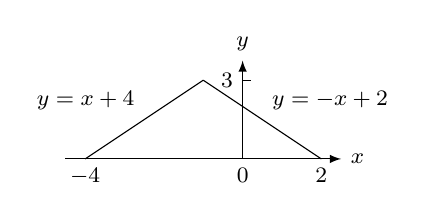
\begin{tikzpicture}[font=\footnotesize]
\draw[-latex](-2.25,0)--(1.25,0)node[right]{$x$};
\draw[-latex](0,0)node[below]{$0$}--(0,1.25)node[above]{$y$};
\draw(-2,0)node[below]{$-4$}--(-0.5,1)node[pos=0.5,above left]{$y=x+4$};
\draw(1,0)node[below]{$2$}--(-0.5,1)node[pos=0.5,above right]{$y=-x+2$};
\draw(0,1)node[left]{$3$}--++(0.1,0);
\end{tikzpicture}
\caption{}
\label{شکل_سوال_تکمل_اوسط_قیمت_ترسیم_الف}
\end{minipage}\hfill
\begin{minipage}{0.45\textwidth}
\centering
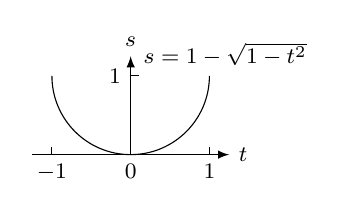
\begin{tikzpicture}[font=\footnotesize]
\draw[-latex](-1.25,0)--(1.25,0)node[right]{$t$};
\draw[-latex](0,0)node[below]{$0$}--(0,1.25)node[above]{$s$};
\draw([shift={(180:1)}]0,1) arc (180:360:1);
\draw(-1,0)node[below]{$-1$}--++(0,0.1)  (1,0)node[below]{$1$}--++(0,0.1)  (0,1)node[left]{$1$}--++(0.1,0);
\draw(1,1)node[above,xshift=2mm]{$s=1-\sqrt{1-t^2}$};
\end{tikzpicture}
\caption{}
\label{شکل_سوال_تکمل_اوسط_قیمت_ترسیم_پ}
\end{minipage}
\end{figure}
\ابتدا{سوال}
وقفہ \عددی{[0,2\pi]} پر تفاعل \عددی{f(t)=\sin t} دیا گیا ہے۔
\انتہا{سوال}
%======================
\ابتدا{سوال}\شناخت{سوال_تکمل_اوسط_قیمت_ترسیم_ب}
وقفہ \عددی{[-\tfrac{\pi}{4},\tfrac{\pi}{4}]} پر تفاعل \عددی{f(\theta)=\tan\theta} دیا گیا ہے۔
\انتہا{سوال}
%========================
\موٹا{نظریہ اور مثالیں}

\ابتدا{سوال}
کم سے کم اور زیادہ سے زیادہ عدم مساوات استعمال کرتے ہوئے درج ذیل کی قیمت کے لئے بالائی اور زیریں حد تلاش کریں۔
$\int_0^1\tfrac{1}{1+x^2}\dif x$
\انتہا{سوال}
%=========================
\ابتدا{سوال}
کم سے کم اور زیادہ سے زیادہ عدم مساوات استعمال کرتے ہوئے درج ذیل کی قیمت کے لئے بالائی اور زیریں حد تلاش کریں۔
\begin{align*}
\int_0^{0.5}\tfrac{1}{1+x^2}\dif x,\quad \int_{0.5}^1\tfrac{1}{1+x^2}\dif x
\end{align*}
انہیں استعمال کرتے ہوئے درج ذیل کی قیمت کا بہتر اندازہ حاصل کریں۔
\begin{align*}
\int_0^1\frac{1}{1+x^2}\dif x
\end{align*}
\انتہا{سوال}
%=========================
\ابتدا{سوال}
دکھائیں کہ \عددی{\int_0^1\sin(x^2)\dif x} کی قیمت کسی صورت \عددی{2} نہیں ہو سکتی ہے۔
\انتہا{سوال}
%==========================
\ابتدا{سوال}
دکھائیں کہ \عددی{\int_0^1\sqrt{x+8}\dif x} کی قیمت \عددی{2\sqrt{2}} اور \عددی{3} کے بیچ پائی جاتی ہے۔
\انتہا{سوال}
%==========================
\ابتدا{سوال}
فرض کریں \عددی{f} استمراری ہے اور \عددی{\int_1^2f(x)\dif x=4} دیا گیا ہے۔ دکھائیں کہ \عددی{[1,2]} پر کم از کم ایک بار \عددی{f(x)=4}  ہو گا۔
\انتہا{سوال}
%========================
\ابتدا{سوال}
فرض کریں \عددی{[a,b]} پر \عددی{f} اور \عددی{g} استمراری ہیں جہاں \عددی{a\ne b} ہے۔ مزید \عددی{\int_a^b(f(x)-g(x))\dif x=0} دیا گیا ہے۔دکھائیں کہ \عددی{[a,b]} میں کم از کم ایک بار \عددی{f(x)=g(x)} ہو گا۔
\انتہا{سوال}
%=====================
\ابتدا{سوال}\ترچھا{غیر منفی تفاعل کا تکمل}\\
کمتر بلند تر عدم مساوات استعمال کرتے ہوئے درج ذیل دکھائیں جہاں \عددی{f} قابل تکمل ہے۔
\begin{align*}
f(x)\ge 0,\quad [a,b]\quad \stackrel{\text{\RL{سے مراد}}}{\implies} \quad \int_a^ b f(x)\dif x\ge 0
\end{align*} 
\انتہا{سوال}
%===========================
\ابتدا{سوال}\ترچھا{غیر مثبت تفاعل کا تکمل}\\
درج ذیل دکھائیں جہاں \عددی{f} قابل تکمل ہے۔
\begin{align*}
f(x)\le 0,\quad [a,b]\quad \stackrel{\text{\RL{سے مراد}}}{\implies} \quad \int_a^ b f(x)\dif x\le 0
\end{align*} 
\انتہا{سوال}
%============================
\ابتدا{سوال}
عدم مساوات \عددی{\sin x\le x} کسی بھی \عددی{x\ge 0} کے لئے درست ہے۔تکمل \عددی{\int_0^1\sin x\dif x} کی قیمت کی بالائی حد تلاش کریں۔ 
\انتہا{سوال}
%==========================
\ابتدا{سوال}
وقفہ \عددی{(-\tfrac{\pi}{2},\tfrac{\pi}{2})} پر عدم مساوات \عددی{\sec x\ge 1+\tfrac{x^2}{2}} درست ہے۔اس کو استعمال کرتے ہوئے \عددی{\int_0^1\sec x\dif x} کی قیمت کی زیریں حد تلاش کریں۔
\انتہا{سوال}
%=======================
\ابتدا{سوال}
اگر \عددی{[a,b]} پر قابل تکمل \عددی{f} کی عمومی قیمت \عددی{f_{\text{اوسط}}} ہو تب \عددی{[a,b]} پر عدد \عددی{f_{\text{اوسط}}} اور \عددی{f} کے تکمل کی قیمتیں ایک دوسرے جیسی ہوں گی۔ کیا ایسا ہوتا ہے؟ کیا درج ذیل درست ہے؟ اپنے جواب کی وجہ پیش کریں۔
\begin{align*}
\int_a^b f_{\text{اوسط}}\dif x=\int_a^bf\dif x
\end{align*}
\انتہا{سوال}
%=========================
\ابتدا{سوال}
کیا اچھا ہوتا کہ وقفہ \عددی{[a,b]} پر قابل تکمل تفاعل کی اوسط قیمت درج ذیل قواعد پر پورا اترتی۔
\begin{enumerate}[a.]
\item
$(f+g)_{\text{اوسط}}=f_{\text{اوسط}}+g_{\text{اوسط}}$
\item
$(kf)_{\text{اوسط}}=k(f_{\text{اوسط}})$
\item
$f_{\text{اوسط}}\le g_{\text{اوسط}} \quad \text{اگر}\quad f(x)\le g(x)$
\end{enumerate}
\انتہا{سوال}
%=========================
\ابتدا{سوال}
اگر \عددی{\SI{150}{\kilo\meter}} فاصلہ طے کرتے ہوئے آپ کی اوسط رفتار \عددی{\SI{30}{\kilo\meter\per\hour}} اور واپسی اسی راہ کو طے کرتے ہوئے آپ کی اوسط رفتار \عددی{\SI{50}{\kilo\meter\per\hour}} ہو تب دونوں اطراف کو ملا کر آپ کی اوسط رفتار کتنی ہو گی؟
\انتہا{سوال}
%=====================
\ابتدا{سوال}
ایک ڈیم سے \عددی{\SI{10}{\meter\cubed\per\minute}} کی شرح سے \عددی{\SI{1000}{\meter\cubed}} پانی خارج کیا گیا اور اس کے بعد \عددی{\SI{20}{\meter\cubed\per\minute}} کی شرح سے مزید \عددی{\SI{1000}{\meter\cubed}} پانی خارج کیا گیا۔ پانی خارج کرنے کی اوسط شرح دریافت کریں۔
\انتہا{سوال}
%=========================

\حصہ{بنیادی مسئلہ}
اس حصہ میں تکملی احصاء کا بنیادی مسئلہ پیش کیا جائے گا جو تکمل اور تفرق کا تعلق پیش کرتا ہے۔ اس مسئلہ نے  ریاضیات میں بہت زیادہ ترقی کو ممکن بنایا جس نے اگلے دو صدیوں تک سائنس میں ہلچل مچا دی۔انسانی تاریخ میں اس مسئلہ کی دریافت کو سب سے زیادہ اہم تصور کیا جاتا ہے۔ لبنٹز اور نیوٹن نے علیحدہ علیحدہ اس مسئلہ کو دریافت کیا۔

\جزوحصہء{بنیادی مسئلہ، جزو اول}
قابل تکمل تفاعل \عددی{f(t)} کا مقررہ عدد \عددی{a} سے  عدد \عددی{x} تک تکمل  از خود ایک تفاعل \عددی{F} ہو گا جس کی \عددی{x} پر قیمت درج ذیل ہو گی۔
\begin{align}\label{مساوات_تکمل_بنیادی_مسئلہ_الف}
F(x)=\int_a^xf(t)\dif t
\end{align} 
مثال کے طور پر اگر \عددی{f} غیر منفی ہو اور \عددی{a} کے دائیں جانب \عددی{x} پایا جاتا ہو تب \عددی{a} تا \عددی{x} ترسیم کے نیچے رقبہ \عددی{F(x)} ہو گا۔ تکمل کا بالائی حد \عددی{x} ہے اور \عددی{F} کسی بھی حقیقی متغیر کے حقیقی قیمت تفاعل کی طرح ایک تفاعل ہے۔ یوں متغیر \عددی{x} کی ہر قیمت کے لئے \عددی{F(x)} ایک مخصوص قیمت دیگا جو \عددی{a} تا \عددی{x} تفاعل \عددی{f} کا تکمل ہو گا۔  

نئے تفاعل متعارف کرنے کی ایک اہم ترکیب مساوات \حوالہ{مساوات_تکمل_بنیادی_مسئلہ_الف} دیتی ہے جو تفرقی مساوات کا حل بھی دیتی ہے (جس پر کچھ دیر میں غور کیا جائے گا)۔ مساوات \حوالہ{مساوات_تکمل_بنیادی_مسئلہ_الف} کا یہاں ذکر کرنا اس لئے ضروری ہے کہ یہ تکمل اور تفرق کے بیچ تعلق بیان کرتی ہے۔ یوں اگر \عددی{f} کوئی بھی استمراری تفاعل ہو تب \عددی{F} متغیر \عددی{x} کا قابل تفرق تفاعل ہو گا جس کا تفرق \عددی{f} ہو گا۔ اس طرح ہر \عددی{x} پر درج ذیل ہو گا۔
\begin{align*}
\frac{\dif}{\dif x}F(x)=\frac{\dif}{\dif x}\int_a^xf(t)\dif t=f(x)
\end{align*}
یہ تصور اتنا اہم ہے کہ یہ احصاء کے بنیادی مسئلہ کا پہلا جزو دیتا ہے۔

\ابتدا{مسئلہ}\شناخت{مسئلہ_تکمل_بنیادی_مسئلہ_جزو_اول}\موٹا{احصاء کا بنیادی مسئلہ، جزو اول}\\
اگر \عددی{[a,b]} پر \عددی{f} استمراری ہو تب \عددی{[a,b]} کے ہر نقطہ پر \عددی{F(x)=\int_a^xf(t)\dif t} کا درج ذیل تفرق پایا جائے گا۔
\begin{align}\label{مساوات_تکمل_بنیادی_مسئلہ_ب}
\frac{\dif F}{\dif x}=\frac{\dif}{\dif x}\int_a^xf(t)\dif t=f(x),\quad a\le x\le b
\end{align}
\انتہا{مسئلہ}
%==========================

یہ نتیجہ خوبصورت، طاقتور اور حیران کن ہے اور عین ممکن ہے کہ مساوات \حوالہ{مساوات_تکمل_بنیادی_مسئلہ_ب} پوری ریاضیات میں اہم ترین مساوات ہو۔ یہ کہتی ہے کہ ہر استمراری تفاعل \عددی{f} کے لئے  تفرقی مساوات \عددی{\tfrac{\dif F}{\dif x}=f} کا حل موجود ہے۔ یہ کہتی ہے کہ ہر استمراری تفاعل \عددی{f} کسی دوسرے تفاعل، یعنی \عددی{\int_a^xf(t)\dif t}، کا تفرق ہے۔ یہ کہتی ہے کہ ہر استمراری تفاعل کا الٹ تفرق پایا جاتا ہے۔ اور یہ کہتی ہے کہ تکمل اور تفرق کے عمل ایک دوسرے کے الٹ ہیں۔ 

\ابتدا{ثبوت}\موٹا{برائے مسئلہ \حوالہ{مسئلہ_تکمل_بنیادی_مسئلہ_جزو_اول}}\\
ہم تفرق کی تعریف کو تفاعل \عددی{F(x)} پر لاگو کرتے ہوئے اس مسئلہ کو ثابت کرتے ہیں۔یوں  ہم درج ذیل حاصل تقسیم
\begin{align}\label{مساوات_تکمل_بنیادی_مسئلہ_پ}
\frac{F(x+h)-F(x)}{h}
\end{align}
لکھ کر دکھاتے ہیں کہ \عددی{h\to 0} کرتے ہوئے اس کا حد \عددی{f(x)} ملتا ہے۔

مساوات \حوالہ{مساوات_تکمل_بنیادی_مسئلہ_پ} میں \عددی{F(x+h)} اور \عددی{F(x)}  کی تکملی روپ پر کرنے سے شمار کنندہ درج ذیل صورت اختیار کرتا ہے۔
\begin{align*}
F(x+h)-F(x)=\int_a^{x+h}f(t)\dif t-\int_a^xf(t)\dif t
\end{align*}
صفحہ \حوالہصفحہ{قواعد_تکمل_برائے_تکمل} پر جمع پذیری کا قاعدہ برائے تکملات دائیں ہاتھ کی درج ذیل سادہ روپ دیتی ہے
\begin{align*}
\int_x^{x+h}f(t)\dif t
\end{align*}
لہٰذا مساوات \حوالہ{مساوات_تکمل_بنیادی_مسئلہ_پ} درج ذیل صورت اختیار کرتی ہے۔
\begin{gather}
\begin{aligned}\label{مساوات_تکمل_بنیادی_مسئلہ_ت}
\frac{F(x+h)-F(x)}{h}&=\frac{1}{h}[F(x+h)-F(x)]\\
&=\frac{1}{h}\int_x^{x+h}f(t)\dif t
\end{aligned}
\end{gather}
مسئلہ اوسط قیمت برائے قطعی تکملات (مسئلہ \حوالہ{مسئلہ_تکمل_اوسط_قیمت_قطعی_تکملات}) کے تحت مساوات \حوالہ{مساوات_تکمل_بنیادی_مسئلہ_ت} میں دی گئی آخری تعلق کی قیمت، وقفہ \عددی{x} تا \عددی{x+h} پر \عددی{f} کی کسی ایک قیمت کے برابر ہو گی۔یوں اس وقفہ میں کسی عدد \عددی{c} پر درج ذیل ہو گا۔
\begin{align}\label{مساوات_تکمل_بنیادی_مسئلہ_ٹ}
\frac{1}{h}\int_x^{x+h}f(t)\dif t=f(c)
\end{align}
یوں \عددی{h\to 0} کرتے ہوئے \عددی{\tfrac{1}{h}} ضرب تکمل \عددی{\int_x^{x+h}f(t)\dif t} کی قیمت جاننے کی لئے ہم \عددی{h\to 0} کرتے ہوئے \عددی{f(c)} کی قیمت پر نظر رکھتے ہیں۔

جیسے جیسے \عددی{h\to 0} ہوتا ہے ویسے ویسے وقفے کا سر \عددی{x+h} اس کے سر \عددی{x} کے قریب سے قریب ہوتا جاتا ہے جس کی وجہ سے \عددی{c} بھی \عددی{x} کے قریب سے قریب تر ہوتا جاتا ہے۔ چونکہ \عددی{x} پر \عددی{f} استمراری ہے لہٰذا \عددی{f(c)} کی قیمت \عددی{f(x)} کے قریب سے قریب پہنچتی ہے:
\begin{align}\label{مساوات_تکمل_بنیادی_مسئلہ_ث}
\lim_{h\to 0}f(c)=f(x)
\end{align}
دوبارہ شروع سے بات کرتے ہیں۔یوں درج ذیل لکھا جا سکتا ہے۔
\begin{align*}
\frac{\dif F}{\dif x}&=\lim_{h\to 0}\frac{F(x+h)-F(x)}{h}&&\text{\RL{تفرق کی تعریف}}\\
&=\lim_{h\to 0}\frac{1}{h}\int_x^{x+h}f(t)\dif t&&\text{\RL{مساوات \حوالہ{مساوات_تکمل_بنیادی_مسئلہ_ت}}}\\
&=\lim_{h\to 0} f(c)&&\text{\RL{مساوات \حوالہ{مساوات_تکمل_بنیادی_مسئلہ_ٹ}}}\\
&=f(x)&&\text{\RL{مساوات \حوالہ{مساوات_تکمل_بنیادی_مسئلہ_ث}}}
\end{align*}
یوں ثبوت مکمل ہوتا ہے۔
\انتہا{ثبوت}
%=======================

اگر \عددی{f} کی قیمتیں مثبت ہوں تب درج ذیل مساوات
\begin{align*}
\frac{\dif}{\dif x}\int_a^xf(t)\dif t=f(x)
\end{align*}
کی ایک خوبصورت جیومیٹریائی معنی اخذ کی جا سکتی ہے۔چونکہ تب \عددی{a} تا \عددی{x} تفاعل \عددی{f} کا تکمل \عددی{a} تا \عددی{x} محور \عددی{x}  اور \عددی{f} کے بیچ رقبہ ہو گا۔فرض کریں کہ آپ اس رقبہ پر بائیں سے دائیں چلتے ہوئے ایک قالین  بچھاتے ہیں جس کی متغیر چوڑائی \عددی{f(t)} ہو۔ جب قالین نقطہ \عددی{x} سے گزرتا ہے اس لمحہ زمین ڈھانپنے کی شرح \عددی{f(x)} ہو گی (شکل \حوالہ{شکل_تکمل_قالین})۔ 
\begin{figure}
\centering
\begin{tikzpicture}[]
\draw[-latex](-0.25,0)--(4.5,0)node[right]{$t$};
\draw[-latex](0,-0.2)--(0,2)node[above]{$y$};
\draw[name path=kc](0.25,1.25) to [out=-20,in=-145] node[pos=0.4,above]{$y=f(t)$}(4.5,2);
\path[name path=kya](0.5,0)--++(0,2);
\path[name path=ky](3.5,0)--++(0,2);
\draw[name intersections={of=kc and ky}] (intersection-1)++([shift={(-90:0.25)}]0,0.25) arc (-90:160:0.25)coordinate[pos=1](kB);
\draw([shift={(-90:0.25)}]3.5,0.25) arc (-90:160:0.25)coordinate[pos=1](kA);
\fill[white]($(intersection-1)+(0.25,0.25)$)coordinate(kkB)--(kB)--++(0,-1)--++(0.5,0)--(kkB);
\draw(3.5+0.25,0.25)coordinate(kkC)--($(intersection-1)+(0.25,0.25)$)coordinate(kkD);
\draw(3.5,0)node[below]{$x$};
\draw(kA)--(kB);
\draw[name intersections={of=kya and kc}](0.5,0)node[below]{$a$}--(intersection-1);
\draw(2,0.5)node[font=\small]{$S(x)$   \text{رقبہ}};
\end{tikzpicture}
\caption{نقطہ $x$ پر زمین کو قالین شرح $\tfrac{\dif A}{\dif x}=f(x)$ سے ڈھانپتا ہے۔}
\label{شکل_تکمل_قالین}
\end{figure}
\ابتدا{مثال}
\begin{align*}
\frac{\dif}{\dif x}\int_{-\pi}^x\cos t\dif t&=\cos x&&\text{\RL{مساوات \حوالہ{مساوات_تکمل_بنیادی_مسئلہ_ب} میں $f(t)=\cos t$}}\\
\frac{\dif}{\dif x}\int_0^x \frac{1}{1+t^2}\dif t&=\frac{1}{1+x^2}&&\text{\RL{مساوات \حوالہ{مساوات_تکمل_بنیادی_مسئلہ_ب} میں $f(t)=\tfrac{1}{1+t^2}$}}
\end{align*}
\انتہا{مثال}
%=====================
\ابتدا{مثال}
اگر \عددی{y=\int_1^{x^2}\cos t\dif t} ہو تب \عددی{\tfrac{\dif y}{\dif t}} کیا ہو گا؟

حل:\quad
دھیان رہے کہ تکمل کا بالائی حد \عددی{x^2} ہے نا کہ \عددی{x} لہٰذا \عددی{\tfrac{\dif y}{\dif t}} تلاش کرتے ہوئے \عددی{y} کو
\begin{align*}
y=\int_1^u\cos t\dif t \quad \text{اور}\quad u=x^2
\end{align*}
کا مرکب تصور کر کے زنجیری قاعدہ استعمال کرنا ہو گا:
\begin{align*}
\frac{\dif y}{\dif x}&=\frac{\dif y}{\dif u}\frac{\dif u}{\dif x}&&\text{\RL{زنجیری قاعدہ}}\\
&=\frac{\dif}{\dif u}\int_1^u\cos t\dif t\cdot\frac{\dif u}{\dif x}&&\text{\RL{$y$ کا کلیہ پر کیا گیا ہے}}\\
&=\cos u\cdot\frac{\dif u}{\dif x}&&\text{\RL{مساوات \حوالہ{مساوات_تکمل_بنیادی_مسئلہ_ب} میں $f(t)=\cos t$ ہے}}\\
&=\cos x^2\cdot 2x&&u=x^2\\
&=2x\cos x^2&&\text{\RL{جواب کی عمومی صورت}}
\end{align*}
\انتہا{مثال}
%========================
\ابتدا{مثال}
درج ذیل ابتدائی قیمت مسئلہ کو تکمل کی صورت میں لکھیں۔
\begin{align*}
\frac{\dif y}{\dif x}&=\tan x&&\text{\RL{تفرقی مساوات}}\\
y(1)&=5&&\text{\RL{ابتدائی معلومات}}
\end{align*}
حل:\quad
درج ذیل تفاعل
\begin{align*}
F(x)=\int_1^x\tan t\dif t
\end{align*}
\عددی{\tan t} کا الٹ تفرق ہے۔یوں مساوات کا عمومی حل
\begin{align*}
y=\int_1^x\tan u \dif t+C
\end{align*}
ہو گا جہاں مستقل \عددی{C} کی قیمت ابتدائی معلومات سے اخذ ہو گی:
\begin{gather}
\begin{aligned}\label{مساوات_تکمل_تکمل_صفر_حاصل_ہوا}
5&=\int_1^1\tan t\dif t+C&&y(1)=5\\
5&=0+C\\
C&=5
\end{aligned}
\end{gather}
ابتدائی قیمت مسئلے کا حل درج ذیل ہو گا۔
\begin{align*}
y=\int_1^x\tan t\dif t+5
\end{align*}
تفاعل \عددی{F(x)} لکھتے ہوئے ہم نے تکمل کا زیریں حد \عددی{1} کیوں منتخب کیا؟ درحقیقت ہم کسی بھی عدد کو زیریں حد منتخب کر سکتے ہیں لیکن ابتدائی معلومات میں دی گئی  \عددی{x} کی ابتدائی قیمت \عددی{x=1} بہترین انتخاب ہے جس کو استعمال کرتے ہوئے ابتدائی شرط لاگو کرتے ہوئے تکمل کی قیمت صفر حاصل ہوتی ہے (جیسے مساوات \حوالہ{مساوات_تکمل_تکمل_صفر_حاصل_ہوا} میں ہوئی) اور \عددی{C} خود بخود \عددی{y} کی ابتدائی قیمت کے برابر حاصل ہو گی۔ 
\انتہا{مثال}
%=======================

\جزوحصہء{قطعی تکمل کی قیمت کا حصول}
ہم اب احصاء کے بنیادی مسئلے کے  جزو دوم کی بات کرتے ہیں جو قطعی تکمل کی قیمت حاصل کرنے کے بارے میں ہے۔

\ابتدا{مسئلہ}\شناخت{مسئلہ_تکمل_بنیادی_مسئلہ_جزو_دوم}\موٹا{احصاء کا بنیادی مسئلہ، جزو دوم}\\
اگر \عددی{[a,b]} کے ہر نقطہ پر \عددی{f} استمراری ہو اور \عددی{[a,b]} پر \عددی{f} کا الٹ تفرق \عددی{F} ہو تب درج ذیل ہو گا۔
\begin{align}\label{مساوات_تکمل_بنیادی_مسئلہ_جزو_دوم_الف}
\int_a^bf(x)\dif x=F(b)-F(a)
\end{align} 
\انتہا{مسئلہ}
%======================

درج بالا مسئلہ کہتا ہے کہ \عددی{a} تا \عددی{b} استمراری تفاعل \عددی{f} کے تکمل کی قیمت حاصل کرنے کی خاطر ہمیں \عددی{f} کا الٹ تفرق \عددی{F} چاہیے  جس سے قطعی تکمل کی قیمت \عددی{F(b)-F(a)} حاصل ہو گی۔ الٹ تفرق کی موجودگی کو بنیادی مسئلے کا جزو اول یقینی بناتا ہے۔

\ابتدا{ثبوت}\موٹا{برائے مسئلہ \حوالہ{مسئلہ_تکمل_بنیادی_مسئلہ_جزو_دوم}}\\
ہم جانتے ہیں کہ ایک جیسے تفرق رکھنے والے تفاعل میں صرف مستقل کا فرق ممکن ہے۔ ہم جانتے ہیں کہ درج ذیل ایک تفاعل ہے جس کا تفرق \عددی{f} ہے۔
\begin{align*}
G(x)=\int_a^xf(t)\dif t
\end{align*}
یوں اگر \عددی{F} ایسا دوسرا تفاعل ہو جس کا تفرق \عددی{f} ہو تب پورے \عددی{[a,b]} پر درج ذیل ہو گا جہاں \عددی{C} مستقل ہے۔
\begin{align}\label{مساوات_تکمل_بنیادی_مسئلہ_جزو_دوم_ب}
F(x)=G(x)+C
\end{align}
آئیں مساوات \حوالہ{مساوات_تکمل_بنیادی_مسئلہ_جزو_دوم_ب} سے \عددی{F(b)-F(a)} حاصل کرتے ہیں۔
\begin{align*}
F(b)-F(a)&=[G(b)+C]-[G(a)+C]\\
&=G(b)-G(a)\\
&=\int_a^bf(t)\dif t-\int_a^af(t)\dif t\\
&=\int_a^bf(t)\dif t-0=\int_a^bf(t)\dif t
\end{align*}
یوں مساوات \حوالہ{مساوات_تکمل_بنیادی_مسئلہ_جزو_دوم_الف} حاصل ہوتا ہے جس کے ساتھ ثبوت مکمل ہوتا ہے۔
\انتہا{ثبوت}
%=================
\ابتدا{مثال}
\begin{enumerate}[a.]
\item
$\int\limits_0^{\pi}\cos x\dif x=\left.\sin x\right|_0^{\pi}=\sin \pi-\sin 0=0-0=0$
\item
$\int\limits_{-\pi/4}^0\sec x\tan x\dif x=\left.\sec x\right|_{-\pi/4}^0=\sec 0-\sec(-\tfrac{\pi}{4})=1-\sqrt{2}$
\item
\begin{align*}\int\limits_1^4\big(\frac{3}{2}\sqrt{x}-\frac{4}{x^2}\big)\dif x&=\left[x^{\tfrac{3}{2}}+\frac{4}{x}\right]_1^4\\
&=\left[(4)^{\tfrac{3}{2}}+\frac{4}{4}\right]-\left[(1)^{\tfrac{3}{2}}+\frac{4}{1}\right]\\
&=[8+1]-[5]=4
\end{align*}
\end{enumerate}
\انتہا{مثال}
%===================
ہم نے حصہ \حوالہ{حصہ_تکمل_ریمان_مجموعے_اور_قطعی_تکملات} میں \عددی{x} اور \عددی{x^2} کے تکمل کے کلیات دریافت کیے جن کی وضاحت مسئلہ \حوالہ{مسئلہ_تکمل_بنیادی_مسئلہ_جزو_دوم} کرتا ہے۔ ہم اب دیکھ سکتے ہیں کہ \عددی{a} اور \عددی{b} کی علامتوں پر کسی پابندی کے بغیر درج ذیل ہو گا۔
\begin{align*}
\int_a^bx\dif x&=\left.\frac{x^2}{2}\right|_a^b=\frac{b^2}{2}-\frac{a^2}{2}&&\text{\RL{چونکہ $x$ کا الٹ تفرق $\tfrac{x^2}{2}$ ہے}}\\
\int_a^bx^2\dif x&=\left.\frac{x^3}{3}\right|_a^b=\frac{b^3}{3}-\frac{a^3}{3}&&\text{\RL{چونکہ $x^2$ کا الٹ تفرق $\tfrac{x^3}{3}$ ہے}}
\end{align*}

\ابتدا{مثال}\شناخت{مثال_تکمل_ترسیم_اور_محور_کے_بیچ_رقبہ_الف}
تفاعل \عددی{f(x)=x^3-x^2-2x} کی ترسیم اور \عددی{x} محور کے بیچ \عددی{x=-1} تا \عددی{x=2} رقبہ تلاش کریں۔

حل:\quad
پہلے \عددی{f} کے صفر تلاش کرتے ہیں۔چونکہ \عددی{f}کو درج ذیل لکھا جا سکتا ہے
\begin{align*}
f(x)=x^3-x^2-2x=x(x^2-x-2)=x(x+1)(x-2)
\end{align*}
لہٰذا اس کے صفر \عددی{x=0}، \عددی{x=-1} اور \عددی{x=2} ہوں گے جو \عددی{[-1,2]} کو دو خانوں میں تقسیم کرتا ہے (شکل \حوالہ{شکل_مثال_تکمل_ترسیم_اور_محور_کے_بیچ_رقبہ_الف})۔ خانہ \عددی{[-1,0]} میں \عددی{f\ge 0} اور خانہ \عددی{[0,2]} میں \عددی{f\le 0} ہے۔ہم \عددی{f} کا تکمل دونوں ذیلی وقفوں پر علیحدہ علیحدہ حاصل کر کے ان کی مطلق قیمتوں کو جمع کرتے ہیں۔
\begin{align*}
\int_{-1}^0(x^3-x^2-2x)\dif x&=\big[\frac{x^4}{4}-\frac{x^3}{3}-x^2\big]_{-1}^0&&\text{\RL{ذیلی وقفہ $[-1,0]$ پر تکمل}}\\
&=0-\big[\frac{1}{4}+\frac{1}{3}-1\big]=\frac{5}{12}\\
\int_0^2(x^3-x^2-2x)\dif x&=\big[\frac{x^4}{4}-\frac{x^3}{3}-x^2\big]_{0}^2&&\text{\RL{ذیلی وقفہ $[0,2]$ پر تکمل}}\\
&=\big[4-\frac{8}{3}-4\big]-0=-\frac{8}{3}\\
\text{\RL{کل رقبہ}}&=\frac{5}{12}+\abs{-\frac{8}{3}}=\frac{37}{12}
\end{align*}
\انتہا{مثال}
%=======================
\begin{figure}
\centering
\begin{minipage}{0.4\textwidth}
\centering
\begin{tikzpicture}[font=\small,declare function={f(\x)=\x^3-\x^2-2*\x;}]
\begin{axis}[axis on top,clip=false,small,axis lines=middle,xlabel={$x$},ylabel={$y$},xlabel style={at={(current axis.right of origin)},anchor=west},ylabel style={at={(current axis.above origin)},anchor=south},xtick={-1,2},ytick={\empty}]
\addplot[name path=f,smooth,domain=-1.1:2.1]{f(x)}node[left]{$y=x^3-x^2-2x$};
\path[name path=axis](axis cs:-1,0)--(axis cs:2,0);
\addplot[fill=lgray] fill between[of=axis and f];
\draw(axis cs:-0.5,0.2)node[]{$S=\frac{5}{12}$};
\draw(axis cs:1,-0.5)node[]{$S=\abs{-\tfrac{8}{3}}=\tfrac{8}{3}$};
\end{axis}
\end{tikzpicture}
\caption{تفاعل $y=x^3-x^2-2x$ اور $x$ محور کے بیچ رقبہ (مثال \حوالہ{مثال_تکمل_ترسیم_اور_محور_کے_بیچ_رقبہ_الف})۔}
\label{شکل_مثال_تکمل_ترسیم_اور_محور_کے_بیچ_رقبہ_الف}
\end{minipage}\hfill
\begin{minipage}{0.4\textwidth}
\centering
\begin{tikzpicture}[font=\small,declare function={f(\x)=sin(deg(100*pi*\x));}]
\begin{axis}[axis on top,clip=false,small,axis lines=middle,xlabel={$t$},ylabel={$V$},xlabel style={at={(current axis.right of origin)},anchor=south},ylabel style={at={(current axis.above origin)},anchor=south},xtick={0,0.01,0.02},xticklabels={$0$,$\tfrac{1}{100}$,$\tfrac{1}{50}$},ytick={1},yticklabels={$V_{\text{چوٹی}}$},xmax=0.021,scaled x ticks=false,ymax=1.25]
\addplot[domain=0:0.02,smooth]{f(x)}node[pos=0.25,above right]{$V=V_{\text{چوٹی}}\sin 100\pi t$};
\draw[name path=av](axis cs:0,{2/pi})node[left]{$V_{\text{اوسط}}=\tfrac{2V_{\text{چوٹی}}}{\pi}$}--(axis cs:0.01,{2/pi});
\path[name path=axis](axis cs:0,0)--(axis cs:0.01,0);
\addplot[fill=lgray]fill between[of=axis and av];
\end{axis}
\end{tikzpicture}
\caption{گھریلو برقی دباو کی ترسیم۔ نصف چکر کا اوسط $\tfrac{2V_{\text{چوٹی}}}{\pi}$ جبکہ مکمل چکر کا اوسط صفر ہے۔}
\label{شکل_مثال_تکمل_ترسیم_اور_محور_کے_بیچ_رقبہ_ب}
\end{minipage}%
\end{figure}
%========================
\ابتدا{مثال}\شناخت{مثال_تکمل_ترسیم_اور_محور_کے_بیچ_رقبہ_ب}\ترچھا{گھریلو برق}\\
ہمارے گھروں میں بدلتی رو برقی دباو فراہم کی جاتی ہے جس کی نمونہ کشی درج ذیل سائن تفاعل کرتا ہے
\begin{align*}
V=V_{\text{چوٹی}}\sin 100\pi t
\end{align*}
جہاں \عددی{V} اور \عددی{t} کی اکائیاں بالترتیب وولٹ اور سیکنڈ ہیں۔ اس تفاعل کی تعدد \عددی{50} ہرٹز یعنی پچاس چکر فی سیکنڈ ہے۔ مثبت مستقل \عددی{V_{\text{چوٹی}}} کو \اصطلاح{دباو کی چوٹی}\فرہنگ{دباو!چوٹی}\حاشیہب{peak voltage}\فرہنگ{voltage!peak} کہتے ہیں۔

نصف چکر (\عددی{\tfrac{1}{100}} دورانیہ)  پر \عددی{V} کی اوسط قیمت حاصل کرتے ہیں (شکل \حوالہ{شکل_مثال_تکمل_ترسیم_اور_محور_کے_بیچ_رقبہ_ب})۔
\begin{align*}
V_{\text{اوسط}}&=\frac{1}{(\tfrac{1}{100})-0}\int_0^{1/100}V_{\text{چوٹی}}\sin 100\pi t\dif t\\
&=100V_{\text{چوٹی}}\big[-\frac{1}{100\pi}\cos 100\pi t\big]_0^{1/100}\\
&=\frac{V_{\text{چوٹی}}}{\pi}[-\cos \pi+\cos 0]\\
&=\frac{2V_{\text{چوٹی}}}{\pi}
\end{align*}  
\انتہا{مثال}

%========================
مکمل چکر پر گھریلو برقی دباو کی اوسط صفر ہے جو شکل \حوالہ{شکل_مثال_تکمل_ترسیم_اور_محور_کے_بیچ_رقبہ_ب} کو دیکھ کر ظاہر ہے۔ اگر ہم حرکی لچھا معیاری برقی رو پیما سے گھریلو برقی دباو کی پیمائش کریں تو یہ ہمیں صفر وولٹ بتائے گا۔

برقی دباو کی پیمائش موثر طریقہ سے کرنے کی خاطر ہم ایسا آلہ استعمال کرتے ہیں جو برقی دباو کے مربع کی اوسط کے جذر (\عددی{V_{\text{موثر}}})  کی پیمائش کرتا ہو:
\begin{align*}
V_{\text{موثر}}=\sqrt{(V^2)_{\text{اوسط}}}
\end{align*}
چونکہ \عددی{V^2=(V_{\text{چوٹی}})^2\sin^2 100\pi t} کی ایک چکر پر اوسط قیمت درج ذیل ہے
\begin{align}
(V^2)_{\text{اوسط}}=\frac{1}{(1/50)-0}\int_0^{1/50}(V_{\text{چوٹی}})^2\sin^2 100\pi t\dif t=\frac{(V_{\text{چوٹی}})^2}{2}
\end{align}
لہٰذا موثر برقی دباو درج ذیل ہو گی۔
\begin{align}
V_{\text{موثر}}=\sqrt{\frac{(V_{\text{چوٹی}})^2}{2}}=\frac{V_{\text{چوٹی}}}{\sqrt{2}}
\end{align}
گھریلو برقی دباو اور برقی رو کی قیمتوں کا ذکر کرتے ہوئے ان کی موثر قیمتیں بتائی جاتی ہیں۔ یوں \عددی{230} وولٹ بدلتا برقی دباو سے مراد برقی دباو کی موثر قیمت ہے جس کی چوٹی درج ذیل ہو گی جو موثر قیمت سے کافی زیادہ ہے۔
\begin{align*}
V_{\text{چوٹی}}=\sqrt{2}V_{\text{موثر}}=\sqrt{2}\cdot 230=325\quad \text{(وولٹ)}
\end{align*}

\حصہء{سوالات}
\موٹا{تکمل کی قیمت کا حصول}\\
سوال \حوالہ{سوال_تکمل_تلاش_کریں_قیمت_الف} تا سوال \حوالہ{سوال_تکمل_تلاش_کریں_قیمت_ب} میں تکمل کی قیمت تلاش کریں۔

\ابتدا{سوال}\شناخت{سوال_تکمل_تلاش_کریں_قیمت_الف}
$\int\limits_{-2}^0(2x+5)\dif x$
\انتہا{سوال}
%=======================
\ابتدا{سوال}
$\int_{-3}^4(5-\tfrac{x}{2})\dif x$
\انتہا{سوال}
%=======================
\ابتدا{سوال}
$\int_0^4(3x-\tfrac{x^3}{4})\dif x$
\انتہا{سوال}
%=======================
\ابتدا{سوال}
$\int_{-2}^2(x^3-2x+3)\dif x$
\انتہا{سوال}
%=======================
\ابتدا{سوال}
$\int_0^1(x^2+\sqrt{x})\dif x$
\انتہا{سوال}
%=======================
\ابتدا{سوال}
$\int_0^5x^{3/2}\dif x$
\انتہا{سوال}
%=======================
\ابتدا{سوال}
$\int_1^{32}x^{-6/5}\dif x$
\انتہا{سوال}
%=======================
\ابتدا{سوال}
$\int_{-2}^{-1}\tfrac{2}{x^2}\dif x$
\انتہا{سوال}
%=======================
\ابتدا{سوال}
$\int_0^{\pi}\sin x\dif x$
\انتہا{سوال}
%=======================
\ابتدا{سوال}
$\int_0^{\pi}(1+\cos x)\dif x$
\انتہا{سوال}
%=======================
\ابتدا{سوال}
$\int_0^{\pi/3}2\sec^2x\dif x$
\انتہا{سوال}
%=======================
\ابتدا{سوال}
$\int_{\pi/6}^{5\pi/6}\csc^2x\dif x$
\انتہا{سوال}
%=======================
\ابتدا{سوال}
$\int_{\pi/4}^{3\pi/4}\csc\theta\cot\theta\dif\theta$
\انتہا{سوال}
%=======================
\ابتدا{سوال}
$\int_0^{\pi/3}3\sec u\tan u\dif u$
\انتہا{سوال}
%===================
\ابتدا{سوال}
$\int_{\pi/2}^0\tfrac{1+\cos 2t}{2}\dif t$
\انتہا{سوال}
%===================
\ابتدا{سوال}
$\int_{-\pi/3}^{\pi/3}\tfrac{1-\cos 2t}{2}\dif t$
\انتہا{سوال}
%===================
\ابتدا{سوال}
$\int_{-\pi/2}^{\pi/2}(8y^2+\sin y)\dif y$
\انتہا{سوال}
%===================
\ابتدا{سوال}
$\int_{-\pi/3}^{-\pi/4}(4\sec^2t+\tfrac{\pi}{t^2})\dif t$
\انتہا{سوال}
%===================
\ابتدا{سوال}
$\int_1^{-1}(r+1)^2\dif r$
\انتہا{سوال}
%===================
\ابتدا{سوال}
$\int_{-\sqrt{3}}^{\sqrt{3}}(t+1)(t^2+4)\dif t$
\انتہا{سوال}
%===================
\ابتدا{سوال}
$\int_{\sqrt{2}}^1(\tfrac{u^7}{2}-\tfrac{1}{u^5})\dif u$
\انتہا{سوال}
%===================
\ابتدا{سوال}
$\int_{1/2}^1(\tfrac{1}{v^3}-\tfrac{1}{v^4})\dif v$
\انتہا{سوال}
%===================
\ابتدا{سوال}
$\int_1^{\sqrt{2}}\tfrac{s^2+\sqrt{s}}{s^2}\dif s$
\انتہا{سوال}
%===================
\ابتدا{سوال}
$\int_9^4\tfrac{1-\sqrt{u}}{\sqrt{u}}\dif u$
\انتہا{سوال}
%===================
\ابتدا{سوال}
$\int_{-4}^4\abs{x}\dif x$
\انتہا{سوال}
%===================
\ابتدا{سوال}\شناخت{سوال_تکمل_تلاش_کریں_قیمت_ب}
$\int_0^{\pi}\tfrac{1}{2}(\cos x+\abs{\cos x})\dif x$
\انتہا{سوال}
%===================
\موٹا{تکمل کی قیمت کا حصول بذریعہ بدل}\\
سوال \حوالہ{سوال_تکمل_بدل_بنیادی_الف} تا سوال \حوالہ{سوال_تکمل_بدل_بنیادی_ب} میں بدل کی استعمال سے الٹ تفرق حاصل کرتے ہوئے بنیادی مسئلہ کی مدد سے تکمل کی قیمت تلاش کریں۔ 

\ابتدا{سوال}\شناخت{سوال_تکمل_بدل_بنیادی_الف}
$\int_0^1(1-2x)^3\dif x$
\انتہا{سوال}
%=======================
\ابتدا{سوال}
$\int_1^2\sqrt{3x+1}\dif x$
\انتہا{سوال}
%====================
\ابتدا{سوال}
$\int_0^1t\sqrt{t^2+1}\dif t$
\انتہا{سوال}
%====================
\ابتدا{سوال}
$\int_{-1}^2\tfrac{t\dif t}{\sqrt{2t^2+8}}$
\انتہا{سوال}
%====================
\ابتدا{سوال}
$\int_0^{\pi}\sin^2(1+\tfrac{\theta}{2})\dif \theta$
\انتہا{سوال}
%====================
\ابتدا{سوال}
$\int_{3\pi/8}^{\pi/2}\sec^2(\pi-2\theta)\dif \theta$
\انتہا{سوال}
%====================
\ابتدا{سوال}
$\int_0^{\pi}\sin^2\tfrac{x}{4}\cos\tfrac{x}{4}\dif x$
\انتہا{سوال}
%====================
\ابتدا{سوال}\شناخت{سوال_تکمل_بدل_بنیادی_ب}
$\int_{2\pi/3}^{\pi}\tan^3\tfrac{x}{4}\sec^2\tfrac{x}{4}\dif x$
\انتہا{سوال}
%====================
\موٹا{رقبہ}\\
سوال \حوالہ{سوال_تکمل_رقبہ_تلاش_الف} تا سوال \حوالہ{سوال_تکمل_رقبہ_تلاش_ب} میں دیے وقفے پر تفاعل کی ترسیم اور \عددی{x} محور کے بیچ کل رقبہ تلاش کریں۔ 

\ابتدا{سوال}\شناخت{سوال_تکمل_رقبہ_تلاش_الف}
$y=-x^2-2x,\quad -3\le x\le 2$
\انتہا{سوال}
%====================
\ابتدا{سوال}
$y=3x^2-3,\quad -2\le x\le 2$
\انتہا{سوال}
%=========================
\ابتدا{سوال}
$y=x^3-3x^2+2x,\quad 0\le x\le 2$
\انتہا{سوال}
%=========================
\ابتدا{سوال}
$y=x^3-4x,\quad -2\le x\le 2$
\انتہا{سوال}
%=========================
\ابتدا{سوال}
$y=x^{1/3},\quad -1\le x\le 8$
\انتہا{سوال}
%=========================
\ابتدا{سوال}\شناخت{سوال_تکمل_رقبہ_تلاش_ب}
$y=x^{1/3}-x,\quad -1\le x\le 8$
\انتہا{سوال}
%=========================
\begin{figure}
\centering
\begin{minipage}{0.22\textwidth}
\centering
\begin{tikzpicture}[font=\tiny,declare function={f(\x)=1+cos(deg(\x));}]
\begin{axis}[clip=false,width=3.5cm,axis lines=middle,xtick={3.142},xticklabels={$\pi$},ytick={2},xmax=3.42,ymax=2.2,xlabel style={at={(current axis.right of origin)},anchor=west},ylabel style={at={(current axis.above origin)},anchor=south},xlabel={$x$},ylabel={$y$}]
\addplot[name path=f,domain=0:pi]{f(x)}node[pos=0.5,sloped,below]{$y=1+\cos x$};
\draw[name path=ttop](axis cs:0,2)--(axis cs:pi,2)node[pos=0.5,above]{$y=2$};
\addplot[fill=lgray]fill between[of=f and ttop];
\draw(axis cs:pi,2)--(axis cs:pi,0)node[pos=0.5,sloped,above]{$x=\pi$};
\end{axis}
\end{tikzpicture}
\caption{}
\label{شکل_سوال_تکمل_رقبہ_سایہ_دار_الف}
\end{minipage}\hfill
\begin{minipage}{0.22\textwidth}
\centering
\begin{tikzpicture}[font=\tiny,declare function={f(\x)=sin(deg(\x));}]
\begin{axis}[clip=false,width=3.5cm,axis lines=middle,xtick={0.524,2.62}, xticklabels={$\tfrac{\pi}{6}$,$\tfrac{5\pi}{6}$},ytick={1},xmax=3.42,ymax=1.2,xlabel style={at={(current axis.right of origin)},anchor=west},ylabel style={at={(current axis.above origin)},anchor=south},xlabel={$x$},ylabel={$y$}]
\addplot[name path=f,domain=-0.1:pi+0.1]{f(x)}node[pos=0.5,above]{$y=\sin x$};
\draw(axis cs:0.524,{f(0.524)})--(axis cs:0.524,0);
\draw(axis cs:2.62,{f(2.62)})--(axis cs:2.62,0);
\draw[name path=bbot](axis cs:0.524,{f(0.524)})--(axis cs:2.62,{f(2.62)});
\addplot[fill=lgray]fill between[of=f and bbot];
\end{axis}
\end{tikzpicture}
\caption{}
\label{شکل_سوال_تکمل_رقبہ_سایہ_دار_ب}
\end{minipage}\hfill
\begin{minipage}{0.22\textwidth}
\centering
\begin{tikzpicture}[font=\tiny,declare function={f(\x)=sec(deg(\x))*tan(deg(\x));}]
\begin{axis}[axis on top,clip=false,width=3.5cm,axis lines=middle,xtick={-0.786,0.786}, xticklabels={$-\tfrac{\pi}{4}$,$\tfrac{\pi}{4}$},ytick={-1.4142,1.4142},yticklabels={$-\sqrt{2}$,$\sqrt{2}$},xmin=-1,xmax=1,ymin=-1.6,ymax=2,xlabel style={at={(current axis.right of origin)},anchor=west},ylabel style={at={(current axis.above origin)},anchor=south},xlabel={$\theta$},ylabel={$y$}]
\addplot[name path=f,domain=-pi/4:pi/4]{f(x)};
\draw(axis cs:0,-1.5)node[right]{$y=\sec\theta\tan\theta$};
\draw[name path=ttop](axis cs:-0.786,1.4142)--(axis cs:0.786,1.4142);
\addplot[fill=lgray]fill between[of=f and ttop];
\draw(axis cs:-0.786,1.4142)--(axis cs:-0.786,-1.4142);
\end{axis}
\end{tikzpicture}
\caption{}
\label{شکل_سوال_تکمل_رقبہ_سایہ_دار_پ}
\end{minipage}\hfill
\begin{minipage}{0.22\textwidth}
\centering
\begin{tikzpicture}[font=\tiny,declare function={f(\x)=(sec(deg(\x)))^2;}]
\begin{axis}[axis on top,clip=false,width=3.5cm,axis lines=middle,xtick={-0.786,1}, xticklabels={$-\tfrac{\pi}{4}$,$1$},ytick={1,2},xmin=-1,xmax=1.2,ymax=2.5,xlabel style={at={(current axis.right of origin)},anchor=west},ylabel style={at={(current axis.above origin)},anchor=south},xlabel={$t$},ylabel={$y$}]
\addplot[name path=f,domain=-pi/4:0]{f(x)}node[pos=0.5,pin={[pin distance=2mm]-135:{$y=\sec^2t$}}]{};
\addplot[name path=g,domain=0:1]{1-x^2}node[pos=0.5,pin={[pin distance=4mm]-95:{$y=1-t^2$}}]{};
\draw[name path=fa](axis cs:-0.786,2)--(axis cs:0,2);
\draw[name path=ga](axis cs:0,2)--(axis cs:1,2);
\addplot[fill=lgray]fill between[of=f and fa];
\addplot[fill=lgray]fill between[of=g and ga];
\draw(axis cs:1,0)--(axis cs:1,2);
\end{axis}
\end{tikzpicture}
\caption{}
\label{شکل_سوال_تکمل_رقبہ_سایہ_دار_ت}
\end{minipage}
\end{figure}
سوال \حوالہ{سوال_تکمل_رقبہ_سایہ_دار_الف} تا سوال \حوالہ{سوال_تکمل_رقبہ_سایہ_دار_ت} میں سایہ دار رقبہ تلاش کریں۔

\ابتدا{سوال}\شناخت{سوال_تکمل_رقبہ_سایہ_دار_الف}
وقفہ \عددی{0\le x\le \pi} پر تفاعل \عددی{y=1+\cos x} اور \عددی{y=2} کے بیچ رقبہ (شکل \حوالہ{شکل_سوال_تکمل_رقبہ_سایہ_دار_الف})۔
\انتہا{سوال}
%========================
\ابتدا{سوال}\شناخت{سوال_تکمل_رقبہ_سایہ_دار_ب}
وقفہ \عددی{\tfrac{\pi}{6}\le x\le \tfrac{5\pi}{6}} پر \عددی{y=\sin x} اور \عددی{y=\tfrac{1}{2}} کے بیچ رقبہ (شکل \حوالہ{شکل_سوال_تکمل_رقبہ_سایہ_دار_ب})۔
\انتہا{سوال}
%===================
\ابتدا{سوال}\شناخت{سوال_تکمل_رقبہ_سایہ_دار_پ}
وقفہ \عددی{-\tfrac{\pi}{4}\le x\le\tfrac{\pi}{4}} پر \عددی{y=\sec\theta\tan\theta} اور \عددی{y=\sqrt{2}} کے بیچ رقبہ (شکل \حوالہ{شکل_سوال_تکمل_رقبہ_سایہ_دار_پ})۔
\انتہا{سوال}
%===================
\ابتدا{سوال}\شناخت{سوال_تکمل_رقبہ_سایہ_دار_ت}
وقفہ \عددی{-\tfrac{\pi}{4}\le x\le 0} پر \عددی{y=\sec^2t} اور وقفہ \عددی{0\le x\le 1} پر \عددی{y=1-t^2} ہے۔ ان تفاعل اور  \عددی{y=2} کے بیچ رقبہ (شکل \حوالہ{شکل_سوال_تکمل_رقبہ_سایہ_دار_ت})۔
\انتہا{سوال}
%===================
\موٹا{تکمل کا تفرق}
سوال \حوالہ{سوال_تکمل_سے_تفرق_الف} تا سوال \حوالہ{سوال_تکمل_سے_تفرق_ب} میں  (ا) تکمل حل کر کے جواب  کا تفرق لیں، (ب) تکمل سے سیدھا تفرق حاصل کریں۔

\ابتدا{سوال}\شناخت{سوال_تکمل_سے_تفرق_الف}
$\tfrac{\dif}{\dif x}\int_0^{\sqrt{x}}\cos t\dif t$
\انتہا{سوال}
%=====================
\ابتدا{سوال}
$\tfrac{\dif}{\dif x}\int_1^{\sin x}3t^2\dif t$
\انتہا{سوال}
%======================
\ابتدا{سوال}
$\tfrac{\dif}{\dif t}\int_0^{t^4}\sqrt{u}\dif u$
\انتہا{سوال}
%======================
\ابتدا{سوال}\شناخت{سوال_تکمل_سے_تفرق_ب}
$\tfrac{\dif}{\dif \theta}\int_0^{\tan\theta}\sec^2y\dif y$
\انتہا{سوال}
%======================
سوال \حوالہ{سوال_تکمل_تفرق_درکار_ہے_الف} تا سوال \حوالہ{سوال_تکمل_تفرق_درکار_ہے_ب} میں \عددی{\tfrac{\dif y}{\dif x}} تلاش کریں۔

\ابتدا{سوال}\شناخت{سوال_تکمل_تفرق_درکار_ہے_الف}
$y=\int_0^x\sqrt{1+t^2}\dif t$
\انتہا{سوال}
%======================
\ابتدا{سوال}
$y=\int_1^x\tfrac{1}{t}\dif t,\quad x>0$
\انتہا{سوال}
%============================
\ابتدا{سوال}
$y=\int_0^{\sqrt{x}}\sin(t^2)\dif t$
\انتہا{سوال}
%============================
\ابتدا{سوال}
$y=\int_0^{x^2}\cos\sqrt{t}\dif t$
\انتہا{سوال}
%============================
\ابتدا{سوال}
$y=\int_0^{\sin x}\tfrac{\dif t}{\sqrt{1-t^2}},\quad \abs{x}<\tfrac{\pi}{2}$
\انتہا{سوال}
%============================
\ابتدا{سوال}\شناخت{سوال_تکمل_تفرق_درکار_ہے_ب}
$y=\int_0^{\tan x}\tfrac{\dif t}{1+t^2}$
\انتہا{سوال}
%============================
\موٹا{ابتدائی قیمت مسائل}\\
درج ذیل تفاعل سوال \حوالہ{سوال_تکمل_ابتدائی_قیمت_مسئلہ_الف} تا سوال \حوالہ{سوال_تکمل_ابتدائی_قیمت_مسئلہ_ب} میں کسی ایک ابتدائی قیمت مسئلہ حل کرتے ہیں۔ کون سا تفاعل کس مسئلے کو حل کرتا ہے؟ اپنے جواب کی وجہ بیان کریں۔ 
\begin{multicols}{2}
\begin{enumerate}[a.]
\item
$y=\int_1^x\tfrac{1}{t}\dif t-3$
\item
$y=\int_0^x\sec t\dif t+4$
\item
$y=\int_{-1}^x\sec t\dif t+4$
\item
$y=\int_{\pi}^x\tfrac{1}{t}\dif t-3$
\end{enumerate}
\end{multicols}

\ابتدا{سوال}\شناخت{سوال_تکمل_ابتدائی_قیمت_مسئلہ_الف}
$\tfrac{\dif y}{\dif x}=\tfrac{1}{x},\quad y(\pi)=-3$
\انتہا{سوال}
%=================
\ابتدا{سوال}
$y'=\sec x,\quad y(-1)=4$
\انتہا{سوال}
%=================
\ابتدا{سوال}
$y'=\sec x,\quad y(0)=4$
\انتہا{سوال}
%=================
\ابتدا{سوال}\شناخت{سوال_تکمل_ابتدائی_قیمت_مسئلہ_ب}
$y'=\tfrac{1}{x},\quad y(1)=-3$
\انتہا{سوال}
%=================
سوال \حوالہ{سوال_تکمل_ابتدائی_قیمت_حل_تکمل_صورت_الف} تا سوال \حوالہ{سوال_تکمل_ابتدائی_قیمت_حل_تکمل_صورت_ب} میں دیے گئے ابتدائی قیمت مسئلوں کے حل کو تکمل کی صورت میں لکھیں۔

\ابتدا{سوال}\شناخت{سوال_تکمل_ابتدائی_قیمت_حل_تکمل_صورت_الف}
$\tfrac{\dif y}{\dif x}=\sec x,\quad y(2)=3$
\انتہا{سوال}
%====================
\ابتدا{سوال}
$\tfrac{\dif y}{\dif x}=\sqrt{1+x^2},\quad y(1)=-2$
\انتہا{سوال}
%====================
\ابتدا{سوال}
$\tfrac{\dif s}{\dif t}=f(t),\quad s(t_0)=s_0$
\انتہا{سوال}
%====================
\ابتدا{سوال}\شناخت{سوال_تکمل_ابتدائی_قیمت_حل_تکمل_صورت_ب}
$\tfrac{\dif v}{\dif t}=g(t),\quad v(t_0)=v_0$
\انتہا{سوال}
%====================
\موٹا{عملی استعمال}\\
